\documentclass[UTF8,12pt]{ctexbook}

\usepackage[]{ctex}
\usepackage{amsmath,amsthm,amsfonts,amssymb}
\usepackage{geometry}
\usepackage[colorlinks=true]{hyperref}
\usepackage{indentfirst}
\usepackage[center]{titlesec}
\usepackage{graphicx}
\usepackage{esint}
\usepackage{cases}
\usepackage{tikz}
\usepackage{tikz-3dplot}
\usepackage{pgfplots}

\geometry{left=1cm,right=1cm,top=3cm,bottom=3cm}
\title{db的日常笔记}
\date{最后的编译日期:\today}
\author{dbydd}    
\kaishu
\setlength{\parindent}{2em}
\titleformat{\section}[block]{\LARGE\itshape\mdseries}{\arabic{section}}{1em}{}[]
\titleformat{\subsection}[block]{\Large\itshape\mdseries}{\arabic{section}.\arabic{subsection}}{1em}{}[]
\titleformat{\subsubsection}[block]{\large\itshape\mdseries}{\arabic{section}.\arabic{subsection}.\arabic{subsubsection}}{1em}{}[]
\titleformat{\paragraph}[block]{\small\bfseries}{[\arabic{paragraph}]}{1em}{}[]
\setcounter{secnumdepth}{3}
\setcounter{tocdepth}{3}

\newcommand{\limNormal}[1]{\lim\limits_{#1}}
\newcommand{\myLimToZero}{\limNormal{x \to 0}}
\newcommand{\myLimToInf}{\limNormal{x \to \infty}}
\newcommand{\derivative}{^\prime}
\newcommand{\doubleDerivative}{^{\prime\prime}}
\newcommand{\tripleDerivative}{^{\prime\prime\prime}}
\newcommand{\aLotDerivative}[1]{^{(#1)}}
\newcommand{\partialDerivative}[1]{^\prime_{#1}}
\newcommand{\mathCombination}[2]{C_{#1}^{#2}}
\newcommand{\mathPermutation}[2]{P_{#1}^{#2}}
\newcommand{\upDownSum}[2]{\sum\limits_{#2}^{#1}}
\newcommand{\upDownProd}[2]{\prod\limits_{#2}^{#1}}
\newcommand{\fDerivative}[1]{\fint\derivative(#1)}
\newcommand{\defFunction}[1]{f(#1)}
\newcommand{\definiteIntegral}[2]{\int^{#1}_{#2}}
\newcommand{\mathConstant}{\mathbb{C}}
\newcommand{\degree}{^\circ}
\newcommand{\projection}[1]{Prj_{#1}}
\newcommand{\mathRealNumberCollection}{\mathbb{R}}
\newcommand{\bigCase}[1]{\left(#1\right)}
\newcommand{\innerProduct}[2]{\langle#1,#2\rangle}
\newcommand{\transpose}{^T}
\newcommand{\spaceline}{\\\indent}
\newcommand{\directionDerivative}[3]{\left.\cfrac{\partial #1}{\partial #2}\right|_{#3}}
\newcommand{\partialDerivativeFrac}[2]{\cfrac{\partial #1}{\partial #2}}

%  \newcommand{\drawBaseAxis}{
%    \draw[->,color = red] (-5,0) -- (5,0) node[right]{x};
%    \draw[->,color = blue] (0,-5) -- (0,5) node[above]{y};
%    \filldraw(0,0) circle (0.05);
%    \node (center) at (-0.25,-0.25){o};
%    \foreach \x in {0,1,...,8}
%    {
%      \draw[xshift=\x cm] (-4,0) -- (-4,0.1);
%      \draw[yshift=\x cm] (0,-4) -- (0.1,-4);
%      };
%      \foreach \x in {-4,...,-1}
%      \node[below] at(\x,0){\x};
%      \foreach \x in {1,...,4}
%      \node[below] at(\x,0){\x};
%      \foreach \y in {-4,...,-1}
%      \node[left] at(0,\y){\y};
%      \foreach \y in {1,...,4}
%      \node[left] at(0,\y){\y};
%      }

\begin{document}
\pagestyle{empty}{
  \maketitle
  \paragraph{todos}{
    \begin{enumerate}
      \item 誊录纸质笔记
      \item 隐函数存在定理
      \item 重写线性代数
      \item 场论:p10
      \item 补充多个section,计算机图形学,场论等
    \end{enumerate}
  }

  \thispagestyle{empty}
  \tableofcontents
}
\setcounter{page}{1}

\chapter{数学}{

\section{基本概念}{

\subsection{六大基本初等函数}{
  常数函数,幂函数,指数函数,对数函数,三角函数
}%六大基本初等函数结尾

\subsection{介值定理}{

在数学分析中,介值定理(英语:intermediate value theorem,又称中间值定理)描述了连续函数在两点之间的连续性:

假设有一连续函数$\fint:[a,b]\rightarrow \mathbf{R}$, 且假设$\fint(a)<\fint(b)$, 若对任意数$u$满足$\fint(a)<u<\fint(b)$,则存在一点$c,a<c<b$,使得$\fint(c) = u$,当$\fint(a)>\fint(b)$时也有类似叙述

直观的比喻:这代表在$[a,b]$区间上可以画出一条连续曲线,而不让笔离开纸面.
\newline

定理:

假设$I = [a,b]$是一个实数里的闭区间,而$f:I\rightarrow\mathbf{R}$是连续函数,那么其像集$\fint(I)$也是区间.他或者包含$[\fint(a),\fint(b)]$(如果$\fint(b)\leq\fint(a)$).换言之:

$\fint(I)\supseteq[\fint(a),\fint(b)]$.

或:

$\fint(I)\supseteq[\fint(b), \fint(a)]$.

介值定理通常以下述等价的形式表述:假设$f:I\rightarrow\mathbf{R}$是连续函数,且实数$u$满足$\fint(a)<u<\fint(b)$或$\fint(a)>u>\fint(b)$,则存在$c\in(a,b)$使得$\fint(c) = u$

图示:
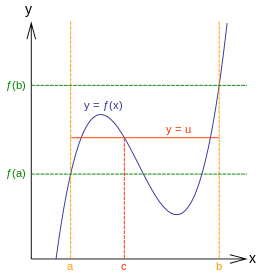
\includegraphics{resources/Intermediatevaluetheorem.png}
}%介值定理结尾

\subsection{二项式定理}{
  $(x + y)^n = x^n + \mathCombination{n - 1}{n}(x^{n-1} y) + \mathCombination{n - 2}{n}(x^{n-2} y^2) + \dots + y^n$
}%二项式定理结尾

\subsection{排列组合}{

  排列:$\mathPermutation{m}{n} = \cfrac{m!}{(m-n)!}$

  组合:$\mathCombination{m}{n} = \cfrac{\mathPermutation{m}{n}}{m!} = \cfrac{n!}{m!(n-m)!}$
}%排列组合结尾

\subsection{韦达定理}{
\subsubsection{韦达定理的普遍情况}{
设$P(x) = a_nx^n + a_{n-1}x^{n-1} + \dotsm + a_1x + a_0$是一个一元n次实(或复)系数多项式,首项系数$a_n \neq 0$,令P的n个根为$x_1,x_2,\dots,x_n$,则根$\{x_i\}$和系数$\{a_j\}$之间满足关系式 :

$$
  \begin{cases}
    x_1 + x_2 + \dotsm + x_{n-1} + x_n = -\cfrac{a_{n-1}}{a_n}                                                           \\
    (x_1x_2 + x_1x_3 + \dotsm + x_1x_n) + (x_2x_3 + x_2x_4 + \dotsm + x_2x_n) + \dotsm + x_{n-1}x = \cfrac{a_{n-2}}{a_n} \\
    \vdots                                                                                                               \\                                                                                                               \\
    x_1x_2 \dotsm x_n = (-1)^n\cfrac{a_n}{a_n}
  \end{cases}
$$

等价的说,对任何$k = 1,2,\dots,n$,系数比$\cfrac{a_{n-k}}{a_n}$是所有任取k个根的乘积的和的$(-1)^k$倍,即 :

$\sum\limits_{1 \leq i_1 < i_2 < \dotsm < i_k \leq n}x_{i_{1}}x_{i_{2}} \dotsm x_{i_{k}} = (-1)^k\cfrac{a_{n-k}}{a_n}$

其中$i_1 < i_2 < \dotsm < i_k$是要让所有根的组合都恰好出现一次.

(等号的左边被称作是初等对称多项式)
}%韦达定理的普遍情况结尾

\subsubsection{n = 2的情况(二次)}{
  设$x_1,x_2$是一元二次多项式$ax^2 + bx + c$的两根,则由$ax^2 +bx + c = a(x - x_1)(x - x_2) = ax^2 - a(x_1 + x_2)x + ax_1x_2$有 :

  $x_1 + x_2 = -\cfrac{b}{a},\qquad x_1x_2 = \cfrac{c}{a}$

  在这个情况下,韦达定理的逆定理同样成立 : 给定一个一元二次多项式$ax^2 + bx + c$,如果有两个数$x_1,x_2$,满足$x_1 + x_2 = -\cfrac{b}{a}$和$x_1x_2 = \cfrac{c}{a}$,则$x_1,x_2$就是多项式$ax^2 + bx + c$的两根.
}%n = 2的情况(二次)结尾

\subsubsection{n = 3的情况(三次)}{
  设$x_1,x_2,x_3$是一元三次多项式$ax^3 + bx^2 + cx + d$的三根,则

  $x_1 + x_2 + x_3 = -\cfrac{b}{a}, x_1x_2 + x_1x_3 + x_2x_3 = \cfrac{c}{a},x_1x_2x_3 = -\cfrac{d}{a}$
}%n = 3的情况(三次)结尾

}%韦达定理结尾

\subsection{极坐标}{
极坐标是不同于笛卡尔坐标系(直角坐标系)的另一种函数图像平面.

极坐标不同于笛卡尔坐标系,他没有x和y轴,而是用基准轴和角度表示一个点.

\subsubsection{极坐标系下的面积}{
  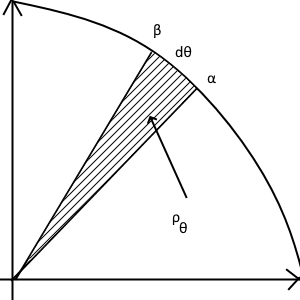
\includegraphics{resources/polar_coordness.png}

  公式为$\cfrac{1}{2}\definiteIntegral{\beta}{\alpha}(p(\theta))^2d\theta$

  p是形成曲线的函数.
  }%极坐标下的面积结尾

  \subsubsection{转换公式}{
    从笛卡尔坐标系到极坐标有一套转换公式.

    $$
      \begin{cases}
        x = \rho\cos\theta \\
        y = \rho\sin\theta
      \end{cases}
    $$
  }%转换公式结尾

}%极坐标结尾

\subsection{不等式}{

\subsubsection{基本不等式}{
  $\cfrac{a + b}{2} \geq \sqrt{ab}$

  注:当且仅当$a = b$时取等号

  其中$\cfrac{a+b}{2}$称为$a,b$的算数平均数,$\sqrt{ab}$称为$a,b$的几何平均数.

  将其变形,可得:
  \begin{enumerate}
    \item $a + b \geq 2\sqrt{ab}$(当且仅当$a = b$时取等号)
    \item $\cfrac{b}{a} + \cfrac{a}{b} \geq 2$($a,b$同号)
    \item $ab \leq (\cfrac{a + b}{2})^2$($a,b\in\mathRealNumberCollection$)
    \item $(\cfrac{a + b}{2})^2 \leq \cfrac{a^2 + b^2}{2}$($a,b\in\mathRealNumberCollection$)
  \end{enumerate}
}%基本不等式结尾


\subsubsection{柯西不等式}{
  柯西不等式有很多种形式:
  \begin{itemize}
    \item {
          二维形式:

          由$(a^2 + b^2)(c^2 + d^2)\geq(ac + bd)^2$变形:$ac + bd \leq \sqrt{(a^2 + b^2)(c^2 + d^2)}$

          当且仅当$ab = cd$(即$\cfrac{a}{c} = \cfrac{b}{d}$)时.

          一般形式为$\upDownSum{n}{i = 1}a_i^2\upDownSum{n}{i = 1}b_i^2\geq\bigCase{\upDownSum{n}{i = 1}a_ib_i)}^2$

          当$\cfrac{a_1}{b_1} = \cfrac{a_2}{b_2} = \dots = \cfrac{a_n}{b_n}$或$a_i,b_i,i = 1,2,3,\dots,n$中至少有一方全为$0$时等号成立.

          一般形式推广:$(x_1 + y_1 + \dots)(x_2 + y_2 + \dots)\dots(x_n + y_n + \dots) \geq \left[\bigCase{\upDownProd{n}{i = 1}x_i}^{\cfrac{1}{n}} + \bigCase{\upDownProd{n}{i = 1}y_i}^{\cfrac{1}{n}} + \dots\right]^n$

          此推广形式又称卡尔松不等式,其表述是:在m×n矩阵中,各列元素之和的几何平均不小于各行元素的几何平均之和.二维形式是卡尔松不等式n=2时的特殊情况.
          }
    \item {
          向量形式:

          对于内积空间中的向量$\vec{x}$和$\vec{y}$,有

          $|\innerProduct{\vec{x}}{\vec{y}}^2| \leq \innerProduct{\vec{x}}{\vec{x}} \times \innerProduct{\vec{y}}{\vec{y}}$

          其中$\innerProduct{\cdot}{\cdot}$表示内积.等价地,将两边开方,等式右边即可以写为两向量范数乘积的形式.

          $|\innerProduct{\vec{x}}{\vec{y}}| \leq ||\vec{x}||\cdot||\vec{y}||$.

          另外,当且仅当$x$和$y$线性相关时,等号成立(仅两个向量而言,线性相关等同于平行).

          若$x_1,\dotsm,x_n \in \mathConstant$和$y_1,\dotsm,y_n \in mathConstant$有虚部,内积即为标注内积.如果用上划线标记共轭复数,这个不等式可以更明确的表述为:

          $|\vec{x_1}\bar{\vec{y_1}} + \dotsm + \vec{x_n}\bar{\vec{y_n}}|^2\leq (|\vec{x_1}|^2 + \dotsm + |\vec{x_n}|^2)(|\vec{y_1}|^2 + \dotsm + |\vec{y_n}|^2)$.
          }
    \item {
          三角形式:

          在三角形$ABC$中,这个式子可以写作:$||\vec{AB}|| + ||\vec{BC}|| \geq ||\vec{AC}||$

          也就是说:$\sqrt{a^2 + b^2} + \sqrt{c^2 + d^2} \geq \sqrt{(a - c)^2 + (b - d)^2}$

          等号成立的条件为:$ad = bc,且ac + bc \geq 0$(即$\cfrac{a}{c} = \cfrac{b}{d}$).
          }
    \item {
          积分形式:

          $\bigCase{\int\defFunction{x}g(x)dx}^2 \leq \int\fint^2(x)dx \int g^2(x)dx$
          }
    \item {
          一般形式:

          设$V$是一线性空间,定义内积,记作$\innerProduct{\alpha}{\beta}$,则:

          $|\innerProduct{\alpha}{\beta}| \leq |\alpha||\beta|$.

          其中$\alpha,\beta$为$V$中的向量.
          }
  \end{itemize}
}%柯西不等式结尾

\subsubsection{均值不等式}{
平均数不等式,或称平均值不等式、均值不等式,是数学上的一组不等式,也是基本不等式的推广.它是说:

如果$x_{1},x_{2},\dotsm,x_{n}$是正数,则:

$\mathbf{H}_n \leq \mathbf{G}_n \leq \mathbf{A}_n \leq \mathbf{Q}_n$

其中:

$\mathbf{H}_n = \cfrac{n}{\upDownSum{n}{i = 1}\cfrac{1}{x_i}} = \cfrac{n}{\cfrac{1}{x_1} + \cfrac{1}{x_2} + \dotsm + \cfrac{1}{x_n}}$

$\mathbf{G}_n = \sqrt[n]{\upDownProd{n}{i = 1}x_i} = \sqrt[n]{x_1x_2\dotsm x_n}$

$\mathbf{A}_n = \cfrac{\upDownSum{n}{i = 1}x_i}{n} = \cfrac{x_1 + x_2 + x_n}{n}$

$\mathbf{Q}_n = \sqrt{\cfrac{\upDownSum{n}{i = 1}x^2_i}{n}} = \sqrt{\cfrac{x^2_1 + x^2_2 + \dotsm + x^2_n}{n}}$

当且仅当$x_1 = x_2 = \dotsm = x_n$,等号成立.

当$n = 2$时:

$\cfrac{2}{\cfrac{1}{x_1} + \cfrac{1}{x_2}} = \cfrac{2x_1x_2}{x_1 + x_2}\leq\sqrt{x_1x_2}\leq\cfrac{x_1 + x_2}{2}\leq\sqrt{\cfrac{x_1^2 + x_2^2}{2}}$

即对这些正数:调和平均数$\leq$几何平均数$\leq$算数平均数$\leq$平方平均数(方均根)

可简记为:“{\bfseries 算几调方}”
}%二元均值不等式结尾  

\subsubsection{算术-几何均值不等式}{
  算术-几何平均值不等式,简称算几不等式,是一个常见而基本的不等式,表现算术平均数和几何平均数之间恒定的不等关系.设$x_1,x_2,\dots,x_n$为$n$个正实数,他们的算数平均数是$\mathbf{A}_n = \cfrac{x_1 + x_2 + \dotsm + x_n}{n}$,他们的几何平均数是$\mathbf{G}_n = \sqrt[n]{x_1\cdot x_2 \dotsm x_n}$.算术-几何平均值不等式表明,对任意的正实数$x_1,\dotsm,x_n$,总有:

  \begin{center}
    $\mathbf{A}_n\geq\mathbf{G}_n$
  \end{center}

  等号当且仅当$x_1 = x_2 = \dotsm = x_n$时成立.

}%算术-几何均值不等式结尾

\subsubsection{常用不等式}{
  \begin{itemize}
    \item $a^2 + b^2 \geq \cfrac{1}{2}(a + b)^2$
    \item $a^2 + b^2 \geq 2ab$
    \item $ab \leq \cfrac{a^2 + b^2}{2}$
    \item $ab \leq (\cfrac{a + b}{2})^2$
    \item $a + b \geq 2\sqrt{ab}$
    \item $a + b \leq \sqrt{2(a^2 + b^2)}$
  \end{itemize}
}%常用不等式结尾

}%不等式结尾

\subsection{零散的定义}{
  \begin{enumerate}
    \item 有界:$\exists\epsilon,f(x) < \epsilon\quad(-\infty < x < \infty )$
  \end{enumerate}
}%零散的定义结尾

\subsection{零散的思想}{
  \begin{enumerate}
    \item 正变换是数学的重要工具,三角变换是只变其形不变其质的.三角变换常常先寻找式子所包含的各个角之间的联系,并以此为依据选择可以联系它们的适当公式,通过换元法把三角恒等变换问题转化为代数恒等变换问题.
  \end{enumerate}
}%零散的思想结尾

}%基本概念结尾

\section{三角函数}{
三角函数一般由单位圆引出,如下:

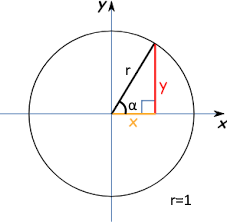
\includegraphics{resources/UnitCircle.png}

\subsection{正三角函数}{
  $\sin{\alpha} = \cfrac{y}{r}$

  $\cos{\alpha} = \cfrac{x}{r}$

  $\tan{\alpha} = \cfrac{y}{x}$
}%正三角函数结尾

\subsection{反三角函数}{
  $\cot{\alpha} = \cfrac{1}{\tan{\alpha}}$

  $\sec{\alpha} = \cfrac{1}{\cos{\alpha}}$

  $\csc{\alpha} = \cfrac{1}{\sin{\alpha}}$
}%反三角函数结尾

\subsection{和差化积}{
  $\sin{\alpha}+\sin{\beta} = 2\sin{\cfrac{\alpha + \beta}{2}}\cos{\cfrac{\alpha - \beta}{2}}$

  $\cos{\alpha}+\cos{\beta} = 2\cos{\cfrac{\alpha + \beta}{2}\cos{\cfrac{\alpha-\beta}{2}}}$

  $\cos{\alpha}-\cos{\beta} = -2\sin{\cfrac{\alpha + \beta}{2}}\cos{\cfrac{\alpha - \beta}{2}}$

  $\sin{\alpha}-\sin{\beta} = 2\sin{\cfrac{\alpha + \beta}{2}}\cos{\cfrac{\alpha - \beta}{2}}$

  $\tan\alpha - \tan\beta = \tan(\alpha - \beta) \cdot (1 + \tan\alpha\tan\beta)$
}%和差化积结尾

\subsection{积化和差}{
  $\cos(\alpha + \beta) = \cos{\alpha}\cos{\beta} - \sin{\alpha}\sin{\beta}$

  $\cos(\alpha - \beta) = \cos{\alpha}\cos{\beta} + \sin{\alpha}\sin{\beta}$

  $\sin(\alpha \pm \beta) = \sin{\alpha}\cos{\beta} \pm \cos{\alpha}\sin{\beta}$

  $\tan(\alpha + \beta) = \cfrac{\tan\alpha + \tan\beta}{1 - \tan\alpha\tan\beta}$

  $\tan(\alpha - \beta) = \cfrac{\tan\alpha - \tan\beta}{1 + \tan\alpha\tan\beta}$

  $\sin{\alpha}\cos{\beta} = \cfrac{1}{2}[\sin{(\alpha + \beta)} + \sin{(\alpha - \beta)}]$

  $\cos{\alpha}\cos{\beta} = \cfrac{1}{2}[\cos{(\alpha + \beta)} + \cos{(\alpha - \beta)}]$

  $\sin{\alpha}\sin{\beta} = -\cfrac{1}{2}[\cos{(\alpha + \beta)} - \cos{(\alpha - \beta)}]$
}%积化和差结尾

\subsection{诱导公式}{
  \indent 奇变偶不变,符号看象限.
  \subsubsection{第一组诱导公式}{
    $\sin{(2k\pi + \alpha)} = \sin{\alpha}$

    $\cos{(2k\pi + \alpha)} = \cos{\alpha}$

    $\tan(2k\pi + \alpha) = \tan\alpha$

    $\cot(2k\pi + \alpha) = \cot\alpha$
  }%第一组诱导公式结尾

  \subsubsection{第二组诱导公式}{
    $\sin(-\alpha) = -\sin\alpha$

    $\cos(-\alpha) = \cos\alpha$

    $\tan(-\alpha) = -\tan\alpha$

    $\cot(-\alpha) = -\cot\alpha$
  }%第二组诱导公式结尾

  \subsubsection{第三组诱导公式}{
    $\sin(\pi + \alpha) = -\sin\alpha$

    $\cos(\pi + \alpha) = -\cos\alpha$

    $\tan(\pi + \alpha) = \tan\alpha$

    $\cot(\pi + \alpha) = \cot\alpha$
  }%第三组诱导公式结尾

  \subsubsection{第四组诱导公式}{
    $\sin(\pi - \alpha) = \sin\alpha$

    $\cos(\pi - \alpha) = -\cos\alpha$

    $\tan(\pi - \alpha) = -\tan\alpha$

    $\cot(\pi - \alpha) = -\cot\alpha$
  }%第四组诱导公式结尾

  \subsubsection{第五组诱导公式}{
    $\sin(\cfrac{\pi}{2} - \alpha) = \cos\alpha$

    $\cos(\cfrac{\pi}{2} - \alpha) = \sin\alpha$

    $\tan(\cfrac{\pi}{2} - \alpha) = \cot\alpha$

    $\cot(\cfrac{\pi}{2} - \alpha) = \tan\alpha$
  }%第五组诱导公式结尾

  \subsubsection{第六组诱导公式}{
    $\sin(\cfrac{\pi}{2} + \alpha) = \cos\alpha$

    $\cos(\cfrac{\pi}{2} + \alpha) = -\sin\alpha$

    $\tan(\cfrac{\pi}{2} + \alpha) = -\cot\alpha$

    $\cot(\cfrac{\pi}{2} + \alpha) = -\tan\alpha$
  }%第六组诱导公式结尾

  \subsubsection{杂项}{
    $a\sin\alpha + b\cos\alpha = \sqrt{a^2 + b^2}\sin(\alpha+\beta)$

    $\cos\alpha = 2cos^2\cfrac{\alpha}{2} - 1 = 1-2\sin^2\cfrac{\alpha}{2}$
  }%杂项结尾

}%诱导公式结尾

\subsection{倍角公式}{

  \subsubsection{二倍角公式}{
    二倍角公式:由两角和公式推出

    $\sin2\alpha = 2\sin\alpha\cos\alpha$

    $\cos2\alpha = \cos^2\alpha - \sin^\alpha = 2\cos^2\alpha - 1 = 1 - 2\sin^2\alpha$

    $\tan2\alpha = \cfrac{2\tan\alpha}{1 - \tan^2\alpha}$
  }%二倍角公式结尾

  \subsubsection{半倍角公式}{
    半倍角公式:将二倍角公式中的角$2\alpha$看作整体$\beta$,经过变形推出:

    $\sin\cfrac{\alpha}{2} = \pm\sqrt{\cfrac{1 - \cos\alpha}{2}}$

    $\cos\cfrac{\alpha}{2} = \pm\sqrt{\cfrac{1 + \cos\alpha}{2}}$

    $\tan\cfrac{\alpha}{2} = \pm\sqrt{\cfrac{1-\cos\alpha}{1+\cos\alpha}} = \cfrac{\sin\alpha}{1+\cos\alpha} = \cfrac{1-\cos\alpha}{\sin\alpha}$

    $\cot\cfrac{\alpha}{2} = \cfrac{1+\cos\alpha}{\sin\alpha} = \cfrac{\sin\alpha}{1-\cos\alpha}$

    $\sec\cfrac{\alpha}{2} = \cfrac{\pm\sqrt{\cfrac{\sec\alpha - 1}{2\sec\alpha}}2\sec\alpha}{\sec\alpha + 1} = \cfrac{\pm\sqrt{\cfrac{4\sec^3\alpha + \sec^2\alpha}{2\cos\alpha}}}{\sec\alpha + 1}$

    $\csc\cfrac{\alpha}{2} = \cfrac{\pm\sqrt{\cfrac{\sec\alpha - 1}{2\sec\alpha}}2\sec\alpha}{\sec\alpha - 1} = \cfrac{\pm\sqrt{\cfrac{3\sec^3\alpha - \sec^2\alpha}{2\sec\alpha}}}{\sec\alpha - 1}$
  }%半倍角公式结尾

  \subsubsection{n倍角公式}{
    $\cos{n\theta} = \upDownSum{\cfrac{n}{2}}{i = 0}[(-1)^i\mathCombination{2i + 1}{n}\cos^{n - 2i}\theta\sin^{2i}\theta]$

    $\sin{n\theta} = \upDownSum{\cfrac{n}{2}}{i = 0}[(-1)^i\mathCombination{2i + 1}{n}\cos^{n - 2i - 1}\theta\sin^{2i+1}\theta]$
  }%n倍角公式结尾

  \subsubsection{万能替换公式}{
    万能替换公式:尝试将正常的三角函数用半角公式表示时经过变形推出:

    角$\alpha(\alpha \neq 2k\pi + \pi ,k \in \mathbf{z})$的所有三角比都可以用 $\tan\cfrac{\alpha}{2}$表示.这组公式叫做万能替换公式

    $\sin\alpha = \cfrac{2\tan\cfrac{\alpha}{2}}{1+\tan^2\cfrac{\alpha}{2}}$

    $\cos\alpha = \cfrac{1 - \tan^2\cfrac{\alpha}{2}}{1 + \tan^2\cfrac{\alpha}{2}}$

    $\tan\alpha \cfrac{2\tan\cfrac{\alpha}{2}}{1 - \tan^2\cfrac{\alpha}{2}}$
  }%万能替换公式结尾

}%倍角公式结尾

\subsection{三角恒等式}{

  倒数关系:

  $\sin\alpha \cdot \csc\alpha = 1$

  $\cos\alpha \cdot \sec\alpha = 1$

  $\tan\alpha \cdot \cot\alpha = 1$

  商数关系:

  $\tan{x} = \cfrac{\sin{x}}{\cos{x}}$

  $\cot\alpha = \cfrac{\cos x}{\sin x}$

  平方关系:

  $\sin^2\alpha + \cos^2\alpha = 1$

  $1 + \tan^2\alpha = \sec^2\alpha$

  $1 + \cot^2\alpha = \csc^2\alpha$

}%三角恒等式结尾

三角形的边角、面积、和外接圆半径之间有着密切的联系

\subsection{解斜三角形}{
设三角形$\triangle ABC$,角A、B、C的对边为abc,以A为原点$O$建系,总有以下公式:

$\mathbf{S}\triangle_{ABC} = \cfrac{1}{2}AB \cdot CD = \cfrac{1}{2}cb\sin A$,即$\mathbf{S}\triangle_{ABC} = \cfrac{1}{2}bc\sin A$

同理得:$\mathbf{S}\triangle_{ABC} = \cfrac{1}{2}\sin B, \mathbf{S}\triangle_{ABC} = \cfrac{1}{2}ab\sin C$.

这就是说,三角形的面积等于任意两边与他们夹角正弦值的一半.

\subsubsection{正弦定理}
将$\cfrac{1}{2}bc\sin A = \cfrac{1}{2}ac\sin B = \cfrac{1}{2}ab\sin C$三个公式同除$\cfrac{1}{2}abc$,得:

$\cfrac{\sin A}{a} = \cfrac{\sin B}{b} = \cfrac{\sin C}{c}$, 也可表示为:$\cfrac{a}{\sin A} = \cfrac{b}{\sin B} = \cfrac{c}{\sin C}$

此式表明:在三角形中,各{\bfseries边}与它所对{\bfseries角的正弦}的比相等

当$\angle C = 90\degree$时,由正弦定理可得:$\cfrac{\sin A}{a} = \cfrac{\sin B}{b} = \cfrac{1}{c}$,即$a = c\sin A,B = C\sin B$

并且,做三角形外接圆:

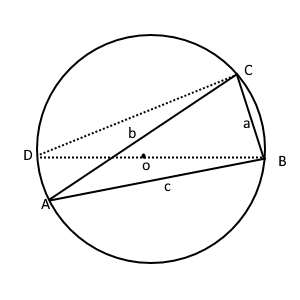
\includegraphics[scale=0.5]{resources/insideTriangleAndCircleOutSide.png}

由圆周角定理可知$\angle D = \angle A,BD = 2R,bc = a$.于是$a = BC = BD\sin A = 2R\sin A$,即:

$\cfrac{a}{\sin A} = 2R$

由正弦定理,可得:$\cfrac{a}{\sin A} = \cfrac{b}{\sin B} = \cfrac{c}{\sin C}$

所以,$a = 2R\sin A,b = 2R\sin B,c = 2R\sin C$

变形也可得到:

$\sin C = \cfrac{c}{2R},\sin B = \cfrac{b}{2R},\sin A = \cfrac{a}{2R}$

以及:

$a^2\sin2B + b^2\sin2A = 2ab\sin C$
}%解斜三角形结尾

\subsubsection{余弦定理}{
  由两点间距离公式,得$a = |BC| = \sqrt{(b\cos A - c)^2 + (b\sin A - 0)^2}$

  两边平方并化简得:

  $a^2 = b^2 - 2b\cos A + c^2$

  $b^2 = a^2 + c^2 - 2ac\cos B$

  $c^2 = a^2 + b^2 - 2ab\cos C$

  也可变形化为:

  $\cos A = \cfrac{b^2 + c^2 - a^2}{2bc}$

  $\cos B = \cfrac{a^2 + c^2 - b^2}{2ac}$

  $\cos C = \cfrac{b^2 + a^2 - c^2}{2ab}$
}%余弦定理结尾
\\

\indent这些关系在直角三角形中也成立.

}%三角函数结尾

\section{空间解析几何}{
  不容小觑且难以理解的部分,加油.

  \subsection{关于向量}{
    在空间解析几何部分不会引入过多有关线性代数的知识(比如向量空间).定理与定义将会互相交织.

    注:本章中的向量默认为三维向量.

    \subsubsection{关于向量的基本概念}{
      有以下概念:
      \begin{itemize}
        \item 数乘:$\lambda \vec{\alpha}$,即$\lambda$倍长度的$\vec{\alpha}$,当$\lambda > 0$时,方向与原向量相同.当$\lambda < 0$时,方向相反.数乘前后向量的起点一致.
        \item 取模:$|\lambda\vec{\alpha}| = |\lambda||\vec{\alpha}|$,前一个“$||$”为绝对值,后一个“$||$”为取模.最后得出的结果为$|\lambda\vec{\alpha}|$的长度.
        \item 单位化:$|\cfrac{\vec{\alpha}}{|\vec{\alpha}|}| = 1$,即将一个向量除以他的长度得到的是单位向量(长度为1的向量)
        \item 在三维标准正交坐标系中存在三个单位向量:$\vec{i},\vec{j},\vec{k}$.他们互相垂直,长度为1.坐标系中任意一点$(x,y,z)$都可以表示为一个向量$\vec{r},\vec{r} = x\vec{i} + y\vec{j} + z\vec{k}$.
        \item 设$\vec{a} = (ax,ay,az),\vec{b} = (bx,by,bz)$.则:$\vec{a} \pm \vec{b} = (ax \pm bx,ay \pm by,az \pm bz)$、$\lambda\vec{a} = (\lambda ax,\lambda ay,\lambda az)$.其中$ax,ay,az,bx,by,bz$称为分量.
        \item 平行:$\vec{b} = \lambda\vec{a},\cfrac{ax}{bx} = \cfrac{ay}{by} = \cfrac{az}{bz}$即:对应分量之比相同.
        \item 向量长度(取模)公式:$\vec{r} = (x,y,z),|\vec{r}| = \sqrt{x^2 + y^2 + z^2}$.注:对于任意维度的向量,取模都是各分量平方和开根号.
        \item 两点之间距离公式:$A:(x_1,y_1,z_1),B:(x_2,y_2,z_2),|\vec{AB}| = \sqrt{(x_1 - x_2)^2 + (y_1 -y_2)^2 + (z_1 - z_2)^2}$.注:在任意维度中,两点之间的距离公式都是对应分量作差的平方和开根号.
        \item {
              两向量夹角:(取锐角)设$\vec{a} = (a_1, a_2, a_3),\vec{b} = (b_1,b_2,b_3)$,设夹角为$\theta$,则:$\cos\theta = \cfrac{|a_1b_1 + a_2b_2 + a_3b_3|}{\sqrt{a_1^2 + a_2^2 + a_3^2}\sqrt{b_1^2 + b_2^2 + b_3^2}}$

              有以下几种情况:
              \begin{enumerate}
                \item 垂直:$a_1b_1 + a_2b_2 + a_3b_3 = 0$
                \item 平行:$\cfrac{a_1}{b_1} = \cfrac{a_2}{b_2} = \cfrac{a_3}{b_3}$
              \end{enumerate}

              求两直线夹角也同理.
              }
      \end{itemize}
    }%关于向量的基本概念结尾

    \subsubsection{方向角与方向余弦}{
      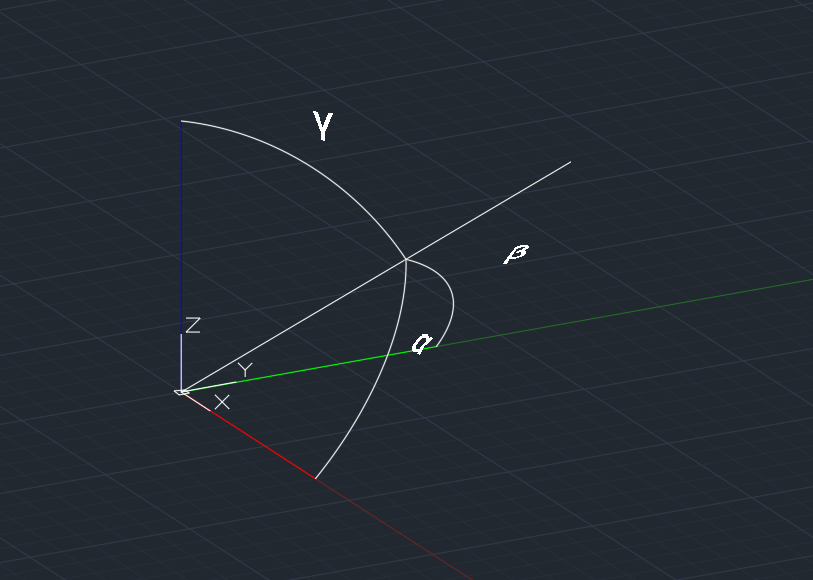
\includegraphics[scale = 0.5]{resources/directionAngle.png}

      $\vec{OM} = \vec{r} = (x,y,z)$

      $\cos\alpha = \cfrac{x}{|\vec{OM}|} = \cfrac{x}{|\vec{r}|}$

      $\cos\beta = \cfrac{y}{|\vec{OM}|} = \cfrac{y}{|\vec{r}|}$

      $\cos\gamma = \cfrac{z}{|\vec{OM}|} = \cfrac{z}{|\vec{r}|}$

      其中$\alpha,\beta,\gamma$称为$\vec{OM}$的方向角.

      有恒等式:$\cos^2\alpha + \cos^2\beta + \cos^2\gamma = 1$

      方向余弦是指在解析几何里,一个向量的三个方向余弦分别是这向量与三个坐标轴之间的角度的余弦.两个向量之间的方向余弦指的是这两个向量之间的角度的余弦.在此处指的是前者,也就是:$\cos\alpha,\cos\beta,\cos\gamma$.

      将方向余弦作为三个分量,即:$(\cos\alpha,\cos\beta,\cos\gamma) = (\cfrac{x}{|\vec{r}|}, \cfrac{y}{|\vec{r}|}, \cfrac{z}{|\vec{r}|}) = \cfrac{1}{|\vec{r}|}\vec{r} = e_r$

      其中$e_r$是个单位向量,表示以向量$\vec{r}$的方向余弦为坐标的向量.

    }%方向角与方向余弦结尾

    \subsubsection{向量投影}{
      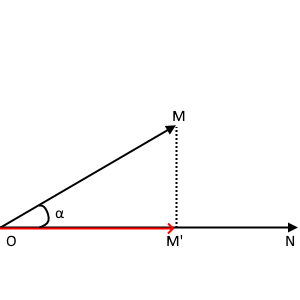
\includegraphics{resources/vector_axis_projection.png}

      直接写出来:
      \begin{enumerate}
        \item $\projection{u}\vec{a} = |\vec{a}|\cdot\cos\alpha$
        \item $\projection{u}(\vec{a} + \vec{b}) = \projection{u}\vec{a} + \projection{u}\vec{b}$
        \item $\projection{u}\lambda\vec{a} = \lambda\projection{u}a$
      \end{enumerate}

      $u$:任意轴\qquad$\vec{a}$:向量\qquad$\projection{u}$:投影到u轴

    }%向量投影结尾

    \subsubsection{数量积/点乘}{
      点乘算出来的是数

      $\vec{a} \cdot \vec{b} = |a|\cdot|b|\cdot\cos\theta = |a|\cdot\projection{a}b = |b|\cdot\projection{b}a$

      $\theta$:夹角\\

      \indent点乘有以下性质:
      \begin{enumerate}
        \item $\vec{a}\cdot\vec{a} = |a|\cdot|a|\cdot\cos0 = |a|^2$
        \item $\vec{a}\cdot\vec{b} = 0,\theta = 90\degree,\vec{a} \perp \vec{b}$\qquad 即:$\vec{a}\cdot\vec{b} = 0 \Leftrightarrow \vec{a} \perp \vec{b}$
        \item $\vec{a}\cdot\vec{b} = \vec{b}\cdot\vec{a}$
        \item $(\vec{a}+\vec{b})\cdot\vec{c} = \vec{a}\cdot\vec{c} + \vec{b}\cdot\vec{c}$
        \item $(\lambda\vec{a})\cdot\vec{b} = \lambda(\vec{a}\cdot\vec{b})$
        \item $\vec{a} = (a_x,a_y,a_z),\vec{b} = (b_x,b_y,b_z),\vec{a}\cdot\vec{b} = a_xb_x + a_yb_y + a_zb_z$
        \item $\cos\theta = \cfrac{\vec{a}\cdot\vec{b}}{|\vec{a}|\cdot|\vec{b}|} = \cfrac{a_xb_x + a_yb_y + a_zb_z}{\sqrt{a_x^2 + a_y^2 + a_z^2}\cdot\sqrt{b_x^2 + b_y^2 + b_z^2}}$
      \end{enumerate}

    }%数量积/点乘结尾

    \subsubsection{向量积/叉乘}{
      叉乘算出来的是向量,这个向量垂直于其他两个向量.右手法则:食指为$\vec{a}$,中指为$\vec{b}$,拇指为$\vec{c}$

      $\vec{a}\times\vec{b} = \vec{c}$

      其中:$\vec{c}\perp\vec{a},\vec{c}\perp\vec{b}$\\

      \indent有以下性质:
      \begin{itemize}
        \item $\vec{a}\times\vec{a} = 0$
        \item 有非零向量$\vec{a},\vec{b},\vec{a}\times\vec{b} = 0\ \Rightarrow \vec{a} // \vec{b}$.即:$\vec{a} // \vec{b} \Leftrightarrow \vec{a} \times \vec{b} = 0$
        \item $\vec{b}\times\vec{a} = -\vec{b}\times\vec{a}$
        \item $(\vec{a} + \vec{b})\times\vec{c} = \vec{a} \times \vec{c} + \vec{b} \times \vec{c}$
        \item $(\lambda\vec{a})\times\vec{b} = \vec{a} \times (\lambda\vec{b}) = \lambda(\vec{a}\times\vec{b})$
      \end{itemize}

      有两种计算方法:

      首先,设$\vec{a} = (a_1,a_2,a_3),\vec{b} = (b_1,b_2,b_3)$,并将结果向量记作$\vec{s}$:

      \begin{itemize}
        \item {
              坐标形式:

              $$
                \vec{s}
                =
                \vec{a}\times\vec{b}
                =
                \begin{bmatrix}
                  s_1 \\
                  s_2 \\
                  s_3
                \end{bmatrix}
                =
                \begin{bmatrix}
                  a_2b_3 - a_3b_2 \\
                  a_3b_1 - a_1b_3 \\
                  a_1b_2 - a_2b_1
                \end{bmatrix}
              $$
              }
        \item {
              行列式形式:

              $$
                \vec{s}
                =
                \vec{a}\times\vec{b}
                =
                \left|\begin{array}{ccc}
                  \vec{i} & \vec{j} & \vec{k} \\
                  a_1     & a_2     & a_3     \\
                  b_1     & b_2     & b_3
                \end{array}\right|
              $$
              }
      \end{itemize}
    }%向量积/叉乘结尾

  }%关于向量结尾

  \subsection{关于空间平面}{

    \subsubsection{空间平面公式}{
      法线向量与平面垂直.\\

      \indent空间平面有以下表示方法:
      \begin{itemize}
        \item {
              点法式:知道一点与法线向量.

              设一点$M_0:(x_0,y_0,z_0)$,法线向量:$\vec{n} = (A,B,C)$

              设$M(x,y,z),\vec{M_0M}=(x - x_0,y - y_0,z - z_0),\vec{n} \cdot \vec{M_0M} = 0$

              平面的点法式方程为:$A(x - x_0) + B(y - y_0) + C(z - z_0) = 0$
              }
        \item {
              一般式:三点确定一个向量.以实例演示:

              设$M_1(2,-1,4),M_2(-1,3,-2),M_3(0,2,3)$代入:

              $Ax + By + Cz + D = 0$

              $$
                \begin{cases}
                  2A - B + 4C = -D \\
                  -A + 3B -2C = -D \\
                  2B + 3C = -D
                \end{cases}
              $$

              也有$Ax + By + Cz + (-Ay_0 - By_0 - Cz_0) = 0$

              (由点法式推出)\\

              \indent有以下情况:
              \begin{enumerate}
                \item $D = 0,Ax + By + Cz = 0$:平面过原点.
                \item $A = 0,By + Cz + D = 0$:平面法线垂直与$x$轴且平行于$x$轴,类似情况同理
                \item $A = B = 0,CZ + D = 0$:平面过$z = -\cfrac{D}{C}$,平行于$xy$轴.
              \end{enumerate}
              }
        \item 截距式:$\cfrac{x}{a} + \cfrac{y}{b} + \cfrac{z}{c} = 1$
      \end{itemize}
    }%关于空间平面结尾

    \subsubsection{求两平面夹角}{
      其实是求两平面法线的夹角(取锐角)

      因此只要设两平面法线向量为$n_1(A_1,B_1,C_1),n_2(A_2,B_2,C_2)$,然后套向量夹角公式就行了.

      其中$\theta = (\widehat{n_1\ n_2})$或$(\widehat{-n_1\ n_2}) = (\pi - (\widehat{n_1\ n_2}))$

      其中当向量平行时意味着平面重合(因为取的是锐角)、
    }%求两平面夹角结尾

    \subsubsection{点到平面距离公式}{
      设点$P_0(x_0,y_0,z_0),Ax + By + Cz + D = 0$

      $d = \cfrac{|Ax_0 + By_0 + Cz_0 + D|}{\sqrt{A^2 + B^2 + C^2}}$
    }%点到平面距离公式结尾

    \subsubsection{直线与平面夹角}{
      指的是直线与法线的夹角

      设与直线同方向的向量$L_1(M,N,P)$,夹角为$\theta$

      $\sin\theta = \cfrac{|AM + BN + CP|}{\sqrt{A^2 + B^2 + C^2}\sqrt{M^2 + N^2 + P^2}}$\\

      \indent有以下几种情况:
      \begin{enumerate}
        \item 直线垂直于平面: $\cfrac{A}{M} = \cfrac{B}{N} = \cfrac{C}{P}$
        \item 直线平行于平面: $AM + BN + CP = 0$
      \end{enumerate}
    }%直线与平面夹角结尾

  }%空间平面及其方程结尾

  \subsection{关于空间直线}{

    \subsubsection{空间直线及其方程}{
      有以下三种形式:

      \begin{enumerate}
        \item {
              一般方程:(即两平面的交线)

              $$
                \begin{cases}
                  A_1x + B_1y + C_1Z + D_1 = 0 \\
                  A_2x + B_2y + C_2z + D_2 = 0
                \end{cases}
              $$
              }
        \item {
              对称式方程:

              设点$M(x,y,z),M_0(x_0,y_0,z_0)$是直线$L$上的任意两点,那么存在向量$\vec{M_0M}$与直线$L$的方向向量$\vec{s}$平行.因此两向量的对应坐标成比例.$(\vec{M_0M} = (x - x_0, y - y_0, z - z_0), \vec{s} = (m,n,p))$,因此得出:

              $\cfrac{x - x_0}{m} = \cfrac{y - y_0}{n} = \cfrac{z - z_0}{p} = t$
              }
        \item {
              参数式:将对称式变形

              $$
                \begin{cases}
                  x = x_0 + mt \\
                  y = y_0 + nt \\
                  z = z_0 + pt
                \end{cases}
              $$
              }
      \end{enumerate}
    }%空间直线及其方程结尾

    \subsubsection{平面束}{
      平面束即形成一条直线的所有面

      $$
        \begin{cases}
          A_1x + B_1y + C_1z + D_1 = 0 \\
          A_2x + B_2y + C_2z + D_2 = 0
        \end{cases}
      $$

      其中$A_1,B_1,C_1$与$A_2,B_2,C_2$不成比例.即:$A_1x + B_1y + C_1z + D_1 + \lambda(A_2x + B_2y + C_2z + D_2) = 0, (\lambda \in \mathRealNumberCollection)$
    }%平面束结尾

  }%关于空间直线结尾

  \subsection{关于空间曲线}{

    \subsubsection{空间曲线及其方程}{
      有以下两种形式:

      \begin{enumerate}
        \item {
              一般式:(两曲面的交线)

              $$
                \begin{cases}
                  F(x,y,z) = 0 \\
                  G(x,y,z) = 0
                \end{cases}
              $$
              }
        \item {
              参数方程:(将曲线上的动点的坐标表示为参数t的函数)

              $$
                \begin{cases}
                  x = x(t) \\
                  y = y(t) \\
                  z = z(t)
                \end{cases}
              $$
              }
      \end{enumerate}
    }%空间曲线及其方程结尾

    \subsubsection{空间曲线在坐标系面上的投影}{

      设空间曲线c的一般方程为:

      $$
        \begin{cases}
          F(x,y,z) = 0 \\
          G(x,y,z) = 0
        \end{cases}
      $$

      消去其中一个变量,(比如z),求在xoy上的投影,得到方程:

      $$
        \begin{cases}
          F(x,y) = 0 \\
          z = 0
        \end{cases}
      $$
    }%空间曲线在坐标系面上的投影结尾

    \subsubsection{空间曲线的切线及法平面}{
      先写出空间曲线的切线方程 :

      $$
        \begin{cases}
          x = \phi(t) \\
          y = \Phi(t) \\
          z = \omega(t)
        \end{cases}
      $$

      其中 $t \in [\alpha,\beta]$,设三个函数都可导且不同时为0.

      则切向量$\vec{T} = \begin{bmatrix}
          \phi\derivative(t_0) & \Phi\derivative(t_0) & \omega\derivative(t_0)
        \end{bmatrix}$

      切线方程为 : $\cfrac{x - x_0}{\phi\derivative(t_0)} = \cfrac{y - y_0}{\Phi\derivative(y_0)} = \cfrac{z - z_0}{\omega\derivative(t_0)}$

      则法平面的点法式方程为 : $\phi\derivative(t_0)(x - x_0) + \Phi\derivative(t_0)(y - y_0) + \omega\derivative(z - z_0) = 0$
    }%空间曲线的切线及法平面

    \subsubsection{空间曲线的切平面及法线}{
      有两种情况 :

      \begin{enumerate}
        \item {
              $F(x,y,z) = 0$(即隐函数)

              则切平面的方程为:$F\derivative_x(x_0,y_0,z_0)(x - x_0) + F\derivative_y(x_0,y_0,z_0)(y - y_0) + F\derivative_z(x_0,y_0,z_0)(z - z_0) = 0$

              法线的方程为 : $\cfrac{x - x_0}{F\derivative_x(x_0,y_0,z_0)} = \cfrac{y - y_0}{F\derivative_y(x_0,y_0,z_0)} = \cfrac{z - z_0}{F\derivative_z(x_0,y_0,z_0)}$
              }
        \item {
              $z = \defFunction{x,y}$,只需让$F = \defFunction{x,y} - z$,然后套公式1.

              切平面解析式为 : $f\derivative_x(x_0,y_0)(x - x_0) + f\derivative_y(x_0,y_0)(y - y_0) - (z - z_0) = 0$
              }
      \end{enumerate}
    }%空间曲线的切平面及法线

  }%关于空间曲线结尾

  \subsection{关于空间曲面}{

    \subsubsection{空间曲面及其方程}{
      有非常多种曲面,都给他列出来:

      \begin{itemize}
        \item {
              旋转曲面:由二次曲线绕某一坐标轴旋转形成.

              \begin{itemize}
                \item {
                      设YOZ平面上有曲线$\defFunction{y,z} = 0$:

                      \begin{itemize}
                        \item 绕z轴旋转,曲面表达式为:$\defFunction{\pm\sqrt{x^2 + y^2},z} = 0$
                        \item 绕y轴旋转,曲面表达式为:$\defFunction{y,\pm\sqrt{x^2 + z^2}} = 0$
                      \end{itemize}
                      }
                \item {
                      设XOY平面上有曲线$\defFunction{x,y} = 0$:

                      \begin{itemize}
                        \item 绕x轴旋转,曲面表达式为:$\defFunction{x,\pm\sqrt{y^2 + z^2}} = 0$
                        \item 绕y轴旋转,曲面表达式为:$\defFunction{\pm\sqrt{x^2 + z^2},y} = 0$
                      \end{itemize}
                      }
                \item {
                      设XOZ平面上有曲线$\defFunction{x,z} = 0$:

                      \begin{itemize}
                        \item 绕x轴旋转,曲面表达式为:$\defFunction{x,\pm\sqrt{y^2 + z^2}} = 0$
                        \item 绕z轴旋转,曲面表达式为:$\defFunction{\pm\sqrt{x^2 + y^2},z} = 0$
                      \end{itemize}
                      }
              \end{itemize}
              }
        \item {
              二次曲面:

              二次曲面有以下12种:
              \begin{itemize}
                \item {
                      椭球面:

                      在直角坐标系中的方程为:

                      $\cfrac{x^2}{a^2} + \cfrac{y^2}{b^2} + \cfrac{z^2}{c^2} = 1$

                      其中a和b是赤道半径(沿着x和y轴),c是极半径,(沿着z轴).这三个数都是固定的正实数,决定了椭球的形状.

                      如果三个半径都是相等的,那么就是一个球;如果有两个半径是相等的,则是一个类球面.

                      \begin{itemize}
                        \item $a = b = c$:球
                        \item $a = b > c$:扁球面
                        \item $a = b < c$:长球面
                        \item $a \neq b,b \neq c,c \neq a$:不等边椭球(三条边都不相等)
                      \end{itemize}

                      点(a,0,0)、(0,b,0)和(0,0,c)都在曲面上.从原点到这三个点的线段,称为椭球的半主轴.它们与椭圆的半长轴和半短轴相对应.

                      体积公式为:$\cfrac{4}{3}\pi abc$.

                      注意,当三个半径都相等时,这个公式便化为球的体积;两个半径相等时,便化为扁球面或长球面的体积.
                      }
                \item {
                      抛物面:

                      例:$y^2 - 2x = 0 / F(x,y) = 0$,参数中缺少z,因此母线平行于z轴
                      }
                \item {
                      椭圆抛物面:

                      椭圆抛物面在直角坐标系中的方程为:$z = \cfrac{x^2}{a^2} + \cfrac{y^2}{b^2}$
                      }
                \item {
                      双曲抛物面:

                      双曲抛物面在直角坐标系中的方程为:$z = \cfrac{x^2}{a^2} - \cfrac{y^2}{b^2}$
                      }
                \item {
                      单叶双曲面:

                      单叶双曲面在直角坐标系中的方程为:$\cfrac{x^2}{a^2} + \cfrac{y^2}{b^2} - \cfrac{z^2}{c^2} = 1$

                      当a = b时双曲面就会变得比较圆
                      }
                \item {
                      双叶双曲面:

                      双叶抛物面在直角坐标系中的方程为:$\cfrac{x^2}{a^2} + \cfrac{y^2}{b^2} - \cfrac{z^2}{c^2} = -1$

                      当a = b时双曲面就会变得比较圆
                      }
                \item {
                      类球面:

                      类球面是一种二次曲面.二维的椭圆有两个主轴,称为长轴与短轴.在三维空间里,将一个椭圆绕着其任何一主轴旋转,则可得到一个类球面.

                      \begin{itemize}
                        \item 假若,这旋转主轴是长轴,则这个类球面为长球面.例如,英式足球里所用的橄榄球是长球形状.
                        \item 假若,这旋转主轴是短轴,则这个类球面为扁球面.例如,地球在北极与南极稍微有点扁平,在赤道又有点凸涨.所以,地球是扁球形状.
                        \item  假若,生成的椭圆是圆圈,则这个类球面为完全对称的圆球面.
                      \end{itemize}

                      用另一种方法来描述,类球面是一种椭球面.而椭球面的公式已经给出,其中a与b分别是椭球面在x轴与y轴的赤道半径,c是椭球面在z轴的极半径,这三个正实数的半径决定了椭球面的形状.以z轴为旋转轴的类球面a = b,他的方程为:

                      $\cfrac{x^2 + y^2}{a^2} + \cfrac{z^2}{c^2} = 1$

                      \begin{itemize}
                        \item 如果三个半径都相等,则此椭球面是圆球面$(a = c)$
                        \item 如果类球面的赤道半径小于极半径,则这是类球面中的长球面.$(a < c)$
                        \item 如果类球面的赤道半径大于极半径,则这是类球面中的扁球面.$(a > c)$
                      \end{itemize}
                      }
                \item {
                      球面:

                      在空间解析几何中,球心为$(x_0,y_0,z_0)$,半径为r的球面是满足以下方程的所有点的轨迹:

                      $(x - x_0)^2 + (y - y_0)^2 + (z - z_0)^2 = r^2$

                      当球心在原点上:$x^2 + y^2 + z^2 = r^2$

                      可化作三元二次方程:$Ax^2 + Ay^2 + Az^2 + Bx + Cy + Dz + G = 0$(平方项系数相同)

                      其中$D^2 + E^2 + F^2 > 4AG$.

                      当满足以上两点时可逆推出一个三元二次方程是否为一个球面

                      (当$D^2 + E^2 + F^2 = 4AG$时是一个点)
                      }
                \item {
                      椭圆锥面(二次锥面):

                      椭圆锥面在直角坐标系中的方程为:$\cfrac{x^2}{a^2} + \cfrac{y^2}{b^2} - \cfrac{z^2}{c^2} = 0$

                      当a = b时就会变成圆锥面.
                      }
                \item {
                      椭圆柱面:

                      椭圆柱面在直角坐标系中的方程为:$\cfrac{x^2}{a^2} + \cfrac{y^2}{b^2} = 1$

                      当a = b时就会变成圆柱面.
                      }
                \item {
                      双曲柱面:

                      双曲柱面在直角坐标系中的方程为:$\cfrac{x^2}{a^2} - \cfrac{y^2}{b^2} = 1$
                      }
                \item {
                      抛物柱面:

                      抛物柱面在直角坐标系中的方程为:$x^2 + 2ay = 0$
                      }
              \end{itemize}
              }
      \end{itemize}
    }%空间曲面及其方程结尾

    \subsubsection{伸缩法}{
      注:伸缩法不是放缩法!

      举例:有$x^2 + y^2 = 1$,沿着y轴伸缩两倍,则伸缩后的方程为:$x^2 + \cfrac{y^2}{4} = 1$.

      也就是说:沿着n轴伸缩,就对变量n进行替换.

      伸缩t倍,就把原变量替换成$\cfrac{n}{t}$
    }%伸缩法结尾
  }%关于空间曲面结尾

 }%空间解析几何结尾

\section{微积分}{
注:本章中的“可积”如果没有特别说明则通常指的是传统意义下的“黎曼可积”.勒贝格积分将放在另一章中.(或者这里也可能)

\subsection{极限}{

  在一元的情况下,可微、可导与连续的关系如下

  \begin{itemize}
    \item 可微是可导的充要条件,即:可微$\Leftrightarrow$可导
    \item 可微和可导都是连续的充分条件,即:可微$\rightarrow$连续、可导$\rightarrow$连续
  \end{itemize}

  而在多元的情况下,可微、可导与连续的关系如下:

  \begin{itemize}
    \item 可微(全微分)是可导和连续的充分条件,即:可微$\Rightarrow$可导、可微$\Rightarrow$连续.
    \item 可导推不出连续.
  \end{itemize}

  \subsubsection{定理}{
    \begin{enumerate}
      \item 函数在一点极限存在的条件是左右极限存在且相等
      \item 洛必达法则:当极限为$\cfrac{0}{0}$或者$\cfrac{\infty}{\infty}$时可上下同时求导,求导后极限不变,每一步都需要重新判断是否依然符合类型
    \end{enumerate}
  }%极限定理结尾

  \subsubsection{重要极限}{
    $\myLimToZero\cfrac{\sin{x}}{x}=1 \to \limNormal{x \to 0}\sin{x} \to x$

    $\myLimToInf(1+\cfrac{1}{x})^x = e$
  }%重要极限结尾  

  \subsubsection{等价无穷小}{
    $\myLimToZero a^x - 1 \approx x\ln{a}$

    $\myLimToZero \arcsin(a)x \approx \sin(a)x \approx (a)x$

    $\myLimToZero \arctan(a)x \approx \tan(a)x \approx (a)x$

    $\myLimToZero \ln1+x \approx x$

    $\myLimToZero e^x \approx 1+x$

    $\myLimToZero \sqrt{1 + x} - \sqrt{1 - x} \approx x$

    $\myLimToZero \tan{x} \approx x$

    $\myLimToZero (1 + ax)^b - 1 \approx abx$

    $\myLimToZero (1+x)^\alpha \approx 1+\alpha x$

    $\myLimToZero 1 - \cos x \approx \cfrac{x^2}{2}$

    $\myLimToZero x - \ln(1 + x) \approx \cfrac{x^2}{2}$

    $\myLimToZero \tan x - x \approx \cfrac{x^3}{3}$

    $\myLimToZero x - \arctan x \approx \cfrac{x^3}{3}$

    $\myLimToZero x - \sin x \approx \cfrac{x^3}{6}$

    $\myLimToZero \arcsin x - x \approx \cfrac{x^3}{6}$

    以上等价无穷小都可以由泰勒公式推出
  }%等价无穷小结尾

}%极限结尾

\subsection{导数}{
  导数是什么?教科书上普遍给出的定义是指:函数图像的斜率变化率曲线,事实上某些观点表示导数也可以理解成是函数对于输入值的敏感程度,即:输入值的变化对应的输出值的变化的剧烈程度.

  导数的标准定义是指$\limNormal{x to x_0}\cfrac{f(x) - f(x_0)}{x - x_0}$\ 或者\ $\limNormal{\Delta x \to x_0}\cfrac{f(x + \Delta x) - f(x)}{\Delta x}$

  值得注意的是:求导是一种线性函数,它满足抽象向量空间的八条准则.

  \subsubsection{求导法则}{
    以下为求导的基本法则:
    \begin{enumerate}
      \item $(u + v)\derivative = u\derivative + v\derivative$
      \item $(u - v)\derivative = u\derivative - v\derivative$
      \item $(uv)\derivative = u\derivative v + uv\derivative$
      \item $(uvw)\derivative = u\derivative vw + uv\derivative w + uvw\derivative$
      \item $(\mathbf{c}v)\derivative = \mathbf{c}(v)\derivative$
      \item $\cfrac{u}{v}\derivative = \cfrac{u\derivative v - uv\derivative}{v^2}$
    \end{enumerate}
    注:反函数的导数等于函数导数的倒数,即——互为倒数的导数相乘依然为1
  }%求导法则结尾

  \subsubsection{复合函数求导}{
    对于复合函数求导,有以下方法:

    $y = \fint(u), u = g(x); \cfrac{dy}{dx} = \cfrac{dy}{du} \cdot \cfrac{du}{dx} = f\derivative(u) \cdot g\derivative(x)$
  }%复合函数求导结尾

  \subsubsection{求导公式表}{
    以下为基本函数的求导公式表,类似线性组合,大多数函数的导数可以由以下公式组合得到.

    $\fint(x) = C, \fint\derivative(x) = 0$

    $\fint(x) = x^n, \fint\derivative(x) = nx^{n-1}$

    $\fint(x) = x, \fint\derivative(x) = 1$

    $\fint(x) = \sin x, \fint\derivative(x) = \cos x$

    $\fint(x) = \cos x, \fint\derivative(x) = -\sin x$

    $\fint(x) = \tan x, \fint\derivative(x) = \sec^2 x$

    $\fint(x) = \sec x, \fint\derivative(x) = \sec x\tan x$

    $\fint(x) = \cot x, \fint\derivative(x) = -\csc^2 x$

    $\fint(x) = \csc x, \fint\derivative(x) = -\csc x\cot x$

    $\fint(x) = \arcsin x, \fint\derivative(x) = \cfrac{1}{\sqrt{1 - x^2}}$

    $\fint(x) = \arccos x, \fint\derivative(x) = -\cfrac{1}{\sqrt{1 - x^2}}$

    $\fint(x) = \arctan x, \fint\derivative(x) = \cfrac{1}{1 + x^2}$

    $\fint(x) = arccotx, \fint\derivative(x) = -\cfrac{1}{1 + x^2}$

    $\fint(x) = a^x, \fint\derivative(x) = a^x\ln x$

    $\fint(x) = \log_a x, \fint\derivative(x) = \cfrac{1}{x\ln a}$

    $\fint(x) = \ln x, \fint\derivative(x)= \cfrac{1}{x}$

    $\fint(x) = e^x, \fint\derivative(x) = e^x$
  }%求导公式表结尾
  \newline

  值得注意的是:
  \begin{enumerate}
    \item 在一维的情况下,可导 $\Leftrightarrow$ 左右导数存在且相等

    \item 可导 $\Rightarrow$ 连续

    \item 连续则不一定可导
  \end{enumerate}

  \subsubsection{线性近似/牛顿法近似函数/求方程解}{
    由导数的另一种定义:$\fDerivative{x} = \limNormal{x \to a}\cfrac{\defFunction{x} - \defFunction{a}}{x - a}$

    当不再取极限的时候等号变成约等于,即:$\fDerivative{x} \approx \cfrac{\defFunction{x} - \defFunction{a}}{x - a}$, 两边移项,可得

    $\defFunction{x} \approx \defFunction{a} + (x-a)\fDerivative{a}$或者$x - a \approx -\cfrac{\defFunction{a}}{\fDerivative{a}}$

    前者被称为线性近似,后者就是牛顿法,其实本质上是同一个公式的不同变形.

    当x和a取值越接近,近似也就越精确,这种方法本质上是取级数展开形式的前两位.

  }%线性近似/牛顿法近似函数/方程解结尾

}%导数结尾

\subsection{偏导数}{

  设$\defFunction{x,y,z} = ax + by + cy + d$

  $\fint\partialDerivative{x}(x,y,z) = a$

  $\fint\partialDerivative{y}(x,y,z) = b$

  $\fint\partialDerivative{z}(x,y,z) = c$

  换言之,偏导就是只把要求偏导的变量看作变量,其他变量看作常量再求导.

  \subsubsection{全微分}{

    $\Delta z = \defFunction{x + \Delta x,y + \Delta y} - \defFunction{x,y}\qquad\Delta z : $ 近似求得

    定义:$\defFunction{x,y}$在定义域内有定义,产生$\Delta x$和$\Delta y$,$\Delta z = \defFunction{x + \Delta x,y + \Delta y} - \defFunction{x,y} = A\Delta x + B\Delta y + O(\rho)$

    其中$A = f\partialDerivative{x}, B = f\partialDerivative{y}, \rho = \sqrt{(\Delta x)^2 + (\Delta y)^2}$

    并且$A,B$是$x$和$y$的函数(此处$x,y$为常量),与$\Delta x$和$\Delta y$(此处$\Delta x, \Delta y$是变量)无关.

    如果能写成此形式,则成此函数在这点可微,且$A\Delta x + B\Delta y$叫做他的全微分.

    记作:$dz$(近似值)$= A\Delta x + B\Delta y \approx \Delta z$(精确值)

  }

}%偏导数结尾

\subsection{微分}{
那么微分(differential)又是什么?微分是一个函数在自变量做无穷小变化时函数值的变化.在形式上确实与导数类似,但不应该与导数混淆.

可以形象化理解,微分就是曲线的切线.给定一个横坐标,我们可以在切线上找到纵坐标.就是这样一个映射.而导数就是这条切线的斜率.

\subsubsection{微分公式}{
  给出以下微分公式,与导数确实类似,但微分和导数是两个不同的映射.他们的定义域都是可微函数,微分的值域是1-form,导数的值域是函数.
  \begin{enumerate}
    \item $d(u \pm v) = du \pm dv$
    \item $d(\mathbf{C}u) = \mathbf{c}du$
    \item $d(uv) = vdu + udv$
    \item $d(\cfrac{u}{v} = \cfrac{vdu + udv}{v^2})$
  \end{enumerate}
}%微分公式结尾

\subsubsection{复合微分}{
  与复合求导类似:

  $y = \fint(u), u = g(x);$

  $dy = y\derivative dx = \fint\derivative(u)du = \fint\derivative{u}g\derivative(x)dx$

  即:$du = dg(x)$
}%复合微分结尾

\subsubsection{罗尔中值定理}{
  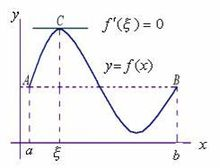
\includegraphics{resources/Rolle's_mean_value_theorem.jpg}

  如果函数$\fint(x)$满足:

  \begin{enumerate}
    \item 在闭区间$[a,b]$上连续;
    \item 在开区间$(a,b)$上可导;
    \item 在区间端点处的函数值相等,即$\fint(a) = \fint(b)$,
  \end{enumerate}

  那么在$(a,b)$内至少有一点$\xi, (a<\xi<b)$,使得$\fint\derivative(\xi) = 0$.这个定理称为罗尔定理
}%罗尔中值定理结尾

\subsubsection{拉格朗日中值定理}{
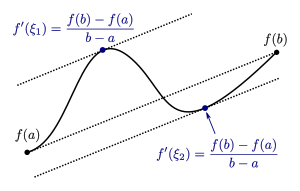
\includegraphics{resources/Lagrange's_mean_value_theorem.png}

令$\fint : [a,b] \to \mathbf{R}$为闭区间$[a,b]$上的一个函数,且在开区间
$(a,b)$内对任意一点$x$,极限$\limNormal{h \to 0}\cfrac{\fint(x + h) - \fint(x)}{h}$存在,
为一个有限数字或者等于$+\infty$或$-\infty$.如果有限,则极限等于$\fDerivative{x}$.

此定理称为{\bfseries拉格朗日中值定理},也简称中值定理,是罗尔中值定理的更一般的形式,同时也是柯西中值定理的特殊情形

这个定理再可以稍微推广一点.只需假设$\fint : [a,b] \to \mathbf{R}$在$[a,b]$连续,且在开区间$(a,b)$内对任意一点$x$,极限$\limNormal{h \to 0}
  \cfrac{\defFunction{x + h} - \defFunction{x}}{b - a}$存在,为一个有限数字或者等于$+\infty$或者$-\infty$.如果有限,则极限等于$\fDerivative{x}$.
这版本定理应用的一个例子是函数$x \to x^{\cfrac{1}{3}}$,实值三次方根函数,其导数在原点趋于无穷.

注意若一个可微函数的值域是复数而不是实数,则上面这定理就未必正确.例如,对实数$x$定义$\defFunction{x} = e^{ix}$.那么

$\defFunction{2\pi} - \defFunction{0} = 0 \neq \fDerivative{c}(2\pi - 0)$

因$|\fDerivative{x}| = 1 \neq 0$时,$c$为开区间$(0,2\pi)$中任意一点.
}%拉格朗日中值定理结尾

\subsubsection{柯西中值定理}{
  柯西中值定理,也叫拓展中值定理,是中值定理的一般形式.它叙述为:如果函数$f$和$g$都在闭区间$[a,b]$上连续,且在开区间$(a,b)$上可微,那么存在某个$c \in (a,b)$,
  使得$(\defFunction{b} - \defFunction{a})g\derivative(c) = (g(b)-g(a))\fDerivative{c}$

  当然,如果$g(a) \neq g(b)$且$g\derivative(c) \neq 0$,则可表示成:$\cfrac{\fDerivative{c}}{g\derivative(c)} = \cfrac{\defFunction{b} - \defFunction{a}}{g(b) - g(a)}$

  在几何上,这表示曲线

  $$
    \begin{cases}
      [a,b] \to \mathbf{R}^2 \\
      t \mapsto (f(t), g(t))
    \end{cases}
  $$
  上存在一点其切线平行于由两点$(\defFunction{a}, g(a))$和$(\defFunction{b}, g(b))$所连接的直线.但柯西定理不能表明在任何情况下这种切线都存在,因为可能存在一些c值使$\defFunction{c} = g(c) = 0$, 所以在这些点曲线根本没有切线.
  下面是这种情况的一个例子

  $t \mapsto (t^3, 1-t^2)$

  在区间$[-1,1]$上,曲线由$(-1, 0)$到$(1,0)$,却并无一个水平切线,然而他在$t = 0$出有一个驻点(实际上是一个尖点).

  柯西中值定理可以用来证明洛必达法则.拉格朗日中值定理是柯西中值定理当$g(t) = t$时的特殊情况.
}%柯西中值定理结尾

}%微分结尾

\subsection{不定积分}{
  在微积分中,函数$\fint$的不定积分(或称反导函数或原函数)是一个可微函数$\mathbf{F}$且其导数等于原来的函数$\fint$,即$F\prime = \fint$.不定积分和定积分的关系由微积分基本定理联系起来.透过微积分基本定理,函数的定积分的计算就可以简单的通过求不定积分来进行.

  \subsubsection{不定积分公式}{
    下面给出不定积分公式:

    \begin{enumerate}
      \item $\int x^adx = \cfrac{x^{a+1}}{a+1} + \mathConstant$
      \item $\int kdx = kx + \mathConstant$
      \item $\int \cfrac{1}{x}dx = \ln(x) + \mathConstant$
      \item $\int \cfrac{dx}{1+x^2}dx = \arctan x + \mathConstant$
      \item $\int \cos xdx = \sin x + \mathConstant$
      \item $\int \sin xdx = -\cos x + \mathConstant$
      \item $\int \cfrac{dx}{\cos^2x} = \int \sec^2xdx = \tan x + \mathConstant$
      \item $\int \cfrac{dx}{\sin^2x} = \int\csc^2xdx = -\cot x + \mathConstant$
      \item $\int \sec x\tan xdx = \sec x + \mathConstant$
      \item $\int \csc x\cot xdx = -\csc x + \mathConstant$
      \item $\int e^xdx = e^x + \mathConstant$
      \item $\int a^xdx = \cfrac{a^x}{\ln a} + \mathConstant$
    \end{enumerate}

  }%不定积分公式结尾

  \subsubsection{不定积分第一类换元积分法}{
    设$\defFunction{x}$为可积函数,$g = g(x)$是连续可导函数,则有:

    $\int \defFunction{g}g\derivative dx = \int \defFunction{g}dg$

    第一类换元积分法基本就是配凑的思想.

  }%不定积分第一类换元积分法结尾

  \subsubsection{不定积分第二类换元积分法}{
    设$\defFunction{x}$为可积函数,$x = x(g)$为连续可导函数,则有:

    $\int \defFunction{x}dx = \int \defFunction{x(g)x\derivative dx}$

  }%不定积分第一类换元积分法结尾.

  \subsubsection{分部积分法}{
    分部积分的公式为:

    $\int udv = uv - \int v du$

    推荐按以下顺序考虑优先代入:

    指数函数、三角函数、幂函数、对数函数、反函数
  }%分部积分法结尾

}%不定积分结尾

\subsection{定积分}{

\subsubsection{定义}{
  $\limNormal{\lambda \to 0}\upDownSum{\infty}{i = 1}\defFunction{\xi_i}\cdot\Delta x_i$

  以上为定义,实际中写法为$\definiteIntegral{a}{b}\defFunction{x}dx$.

  其中$a$为积分区域上限,$b$为积分区域下限.
}%定义结尾

\subsubsection{性质}{
  定积分有以下性质:
  \begin{enumerate}
    \item $\definiteIntegral{a}{b}\defFunction{x}dx = -\definiteIntegral{b}{a}\defFunction{x}dx$即:交换上下限积分结果正负改变.
    \item $a < b < c; \definiteIntegral{b}{a}\defFunction{x}dx = \definiteIntegral{b}{a}\defFunction{x}dx + \definiteIntegral{c}{b}\defFunction{x}dx$,且$\definiteIntegral{b}{a}\defFunction{x}dx = \definiteIntegral{c}{a}\defFunction{x}dx - \definiteIntegral{c}{b}\defFunction{x}dx = \definiteIntegral{c}{a}\defFunction{x}dx + \definiteIntegral{b}{c}\defFunction{x}dx$
    \item $\defFunction{x} \leq g(x); \definiteIntegral{b}{a}\defFunction{x}dx \leq \definiteIntegral{b}{a}g(x)dx$
    \item $|\definiteIntegral{b}{a}\defFunction{x}dx|\leq\definiteIntegral{b}{a}|\defFunction{x}|dx$
  \end{enumerate}
}%性质结尾

\subsubsection{定积分第一类换元积分法}{
  设$\defFunction{x}$为可积函数,$g = g(x)$是连续可导函数,则有:

  $\definiteIntegral{\beta}{\alpha} \defFunction{g}g\derivative dx = \definiteIntegral{g(\beta)}{g(\alpha)} \defFunction{g}dg$
}%定积分第一类换元积分法结尾

\subsubsection{定积分第二类换元积分法}{
  设$\defFunction{x}$为可积函数,$x = x(g)$为连续可导函数,则有:

  $\definiteIntegral{\beta}{\alpha} \defFunction{x}dx = \definiteIntegral{x^{-1}(\beta)}{x^{-1}(\alpha)}\defFunction{x}x\derivative dx$

  简而言之:定积分的第二类换元积分法有两个要点
  \begin{enumerate}
    \item 引入换元函数
    \item 上下限也要变(将原函数上下限代入换元函数)
  \end{enumerate}
}%定积分第二类换元积分法结尾.

\subsubsection{积分上限函数}{
  $I(x) = \definiteIntegral{x}{a}\defFunction{t}dt$

  如果$\defFunction{x}连续$,$I(x)$可导,则$I\prime(x) = \cfrac{d\definiteIntegral{x}{a}f(t)dt}{dx} = f(x)$

  $\defFunction{x}$连续,$I(x)$是$f(x)$的一个原函数.

  有以下几种变体:

  \begin{enumerate}
    \item $(\definiteIntegral{a}{x}\defFunction{t}dt)\prime = -\defFunction{x}$
    \item $(\definiteIntegral{\Phi(x)}{a}\defFunction{t}dt)\prime = \defFunction{\Phi(x)}\Phi\prime(x)$
    \item $[\definiteIntegral{\phi}{\Phi}\defFunction{t}dt]\prime = \defFunction{\phi(x)}\phi\prime(x) - \defFunction{\Phi(x)}\Phi\prime(x)$
  \end{enumerate}

}%积分上限函数结尾

\subsubsection{牛顿-莱布尼兹公式/微积分基本定理}{
  $\definiteIntegral{b}{a}\defFunction{x}dx = F(x)|^b_a = F(b) - F(a)$
}%牛顿-莱布尼兹公式/微积分基本定理结尾

\subsubsection{积分介值定理}{

  在区间$[a,b]$上$m$和$M$分别是$\defFunction{x}$的最小值和最大值.

  $m(b - a) \leq \definiteIntegral{b}{a}\defFunction{x}dx \leq M(b - a)$

}%积分介值定理结尾

\subsubsection{区间再现公式}{
  设$\defFunction{x} = \definiteIntegral{a}{b}g(x)dx$,令$x = a + b - t$,当$x = a$时,$t = b$,当$x = b$时,$t = a$,$dx$变成$-dt$.即:

  $\defFunction{x} = \definiteIntegral{a}{b}g(x)dx = -\definiteIntegral{b}{a}g(a+b-t)dt = \definiteIntegral{a}{b}g(a + b - t)dt$

  由于定积分与被积变量无关,所以将上式结果中的t换成x,与原函数相加,得:

  $\defFunction{x} = \cfrac{1}{2}\definiteIntegral{a}{b}[g(x) + g(a + b - x)]dx$
}%区间再现公式结尾

\subsubsection{积分第一中值定理}{
设$\fint:[a,b] \to \mathbf{R}$为一连续函数,$g:[a,b] \to \mathbf{R}$要求$g(x)$是可积函数且在积分区间不变号,那么存在一点$\xi\in[a,b]$使得:

$\definiteIntegral{b}{a}\defFunction{x}g(x)dx = \defFunction{\xi}\definiteIntegral{b}{a}g(x)dx$
他的几何意义为:

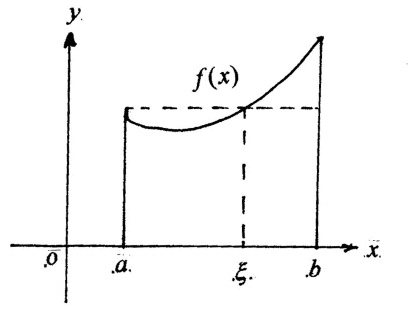
\includegraphics{resources/Geometric_explanation_of_the_mean_value_theorem_for_integration.jpg}
\\\\
以下为证明:

在不失去一般性的条件下,设对所有的$x$,有$g(x) \geq 0$;因为$\fint$是闭区间上的连续函数,$\fint$取得最大值$M$和最小值$m$.于是得出不等式:

$mg(x) \leq \defFunction{x}g(x) \leq Mg(x)$

对不等式求积分,得出:

$m\definiteIntegral{b}{a}g(x)dx \leq \definiteIntegral{b}{a}\defFunction{x}g(x)dx \leq M\definiteIntegral{b}{a}g(x)dx$

如果$\definiteIntegral{b}{a}g(x)dx = 0$,则$\definiteIntegral{b}{a}\defFunction{x}g(x)dx = 0$.$\xi$可以取$[a,b]$上任意一点.

如果不等于$0$,那么$\definiteIntegral{b}{a}g(x)dx>0$,对不等式变形可得:

$m \leq \cfrac{\definiteIntegral{b}{a}\defFunction{x}g(x)dx}{\definiteIntegral{b}{a}g(x)dx} \leq M$

因为$f(x)$是连续函数,所以上面这玩意是个连续函数,所以必定存在一点$\xi\in[a,b]$,使得

$\defFunction{\xi} = \cfrac{\definiteIntegral{b}{a}\defFunction{x}g(x)dx}{\definiteIntegral{b}{a}g(x)dx}$

($g<0$时也可以按这个步骤推出)
\\\\
推论:拉格朗日中值定理的积分形式

在上式中令$g(x) = 1$,则可得出:

设$\fint : [a,b] \to \mathbf{R}$为一连续函数,则$\exists\xi\in[a,b]$,使得

$\defFunction{\xi} = \cfrac{\definiteIntegral{b}{a}\defFunction{x}dx}{b - a}$

也可以由拉格朗日中值定理推出:

设$F(x)$在$[a,b]$上可导,$\defFunction{x} = F\prime(x)$,则$\exists\xi\in[a,b]$,使

$\defFunction{\xi} = F\prime(\xi) = \cfrac{F(b) - F(a)}{b - a} = \cfrac{\definiteIntegral{b}{a}\defFunction{x}dx}{b - a}$

}%积分第一中值定理结尾

\subsubsection{积分第二中值定理}{

积分第二中值定理与积分第一中值定理相互独立,却又是更精细的积分中值定理.

若$f,g$在$[a,b]$上可积且$f(x)$在$[a,b]$上单调,则存在$[a,b]$上的点$\xi$使

$\definiteIntegral{b}{a}\defFunction{x}dx = \defFunction{a}(\xi - a) + \defFunction{b}(b - \xi)$

进而导出:

$\definiteIntegral{\xi}{a}\defFunction{x}dx -\defFunction{a}(\xi - a) = \defFunction{b}(b - \xi) - \definiteIntegral{b}{\xi}\defFunction{x}dx$

他的几何意义很明显为:能找到$\xi\in[a,b]$,使得红色区域的面积和蓝色区域的面积相加等于阴影区域的面积,即S[\uppercase\expandafter{\romannumeral1}] = S[\uppercase\expandafter{\romannumeral2}]

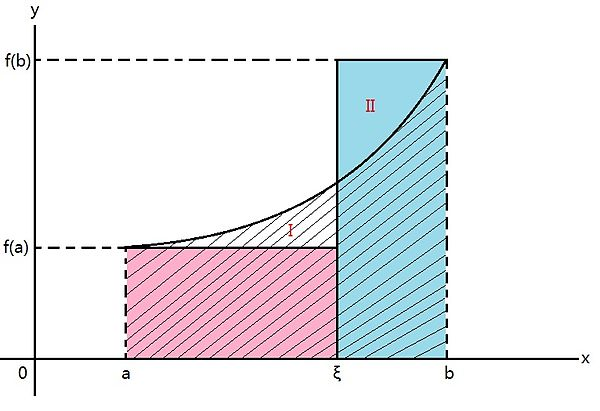
\includegraphics{resources/Geometric_explanation_of_the_second_mean_value_theorem_for_integration.jpg}

}%积分第二中值定理结尾

\subsubsection{定积分求平面函数曲线弧长}{

  $$
    \begin{cases}
      x = \phi(t) \\
      y = \Phi(t)
    \end{cases}
    \alpha \leq t \leq \beta
    \qquad\qquad\qquad\qquad\qquad\qquad\qquad\qquad\qquad\qquad\qquad\qquad
    \begin{cases}
      x = x \\
      y = \defFunction{x}
    \end{cases}
    \alpha \leq t \leq \beta
  $$

  $S = \definiteIntegral{\beta}{\alpha}\sqrt{\phi^{\prime 2}(t) + \Phi^{\prime 2}(t) dt}\qquad\qquad\qquad\qquad\qquad\qquad\qquad\qquad\qquad\qquad\qquad\qquad S = \definiteIntegral{\beta}{\alpha}\sqrt{1 + y^{\prime 2}}$

  极坐标的情况:

  $$
    \begin{cases}
      x = \rho(\theta)\cos\theta \\
      y = \rho(\theta)\sin\theta
    \end{cases}
  $$

  $S = \definiteIntegral{\beta}{\alpha}\sqrt{\rho^{\prime 2}(\theta) + \rho^2(\theta)d\theta}$\qquad(注意求导符号)
}%定积分求平面函数曲线弧长

}%定积分结尾

\subsection{反常积分}{
通常来说只需要极限存在,则此反常积分收敛.

\subsubsection{无穷限反常积分}{

  有以下几种情况:

  \begin{enumerate}
    \item $\definiteIntegral{+\infty}{a}\defFunction{x}dx = \limNormal{b \to +\infty}\definiteIntegral{b}{a}\defFunction{x}dx$
    \item $\definiteIntegral{b}{-\infty}\defFunction{x}dx = \limNormal{t \to -\infty}\definiteIntegral{b}{t}\defFunction{x}dx$
    \item $\definiteIntegral{+\infty}{-\infty}\defFunction{x}dx = \definiteIntegral{0}{-\infty}\defFunction{x}dx + \definiteIntegral{+\infty}{0}\defFunction{x}dx$
  \end{enumerate}
}%无穷限反常积分结尾


\subsubsection{无界函数反常积分}{

  设b为瑕点:

  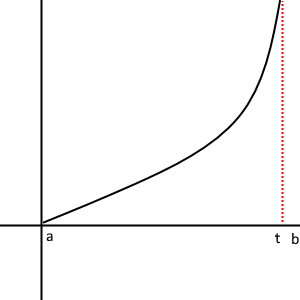
\includegraphics[scale=0.5]{resources/infityFunctionUnormalIntegral.png}

  $\definiteIntegral{b}{a}\defFunction{x}dx = \limNormal{t \to b^-}\definiteIntegral{t}{a}\defFunction{x}dx$

  或者是设a为瑕点:

  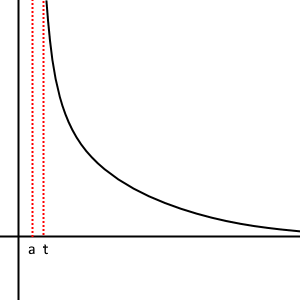
\includegraphics[scale=0.5]{resources/infityFunctionUnormalIntegral2.png}

  $\definiteIntegral{b}{a}\defFunction{x}dx = \limNormal{t \to a^+}\definiteIntegral{b}{t}\defFunction{x}dx$

  或者以上两者情况合一,设c为瑕点将其拆分:

  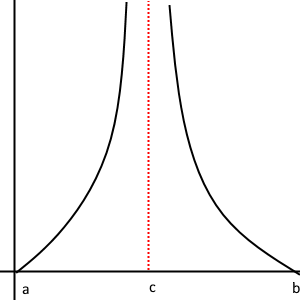
\includegraphics{resources/infityFunctionUnormalIntegral3.png}

  $\definiteIntegral{b}{a}\defFunction{x}dx = \definiteIntegral{c}{a}\defFunction{x}dx + \definiteIntegral{b}{c}\defFunction{x}dx$

  然后按照上方两个情况分别求解.

  依然可以使用牛-莱公式.

  瑕积分换元需要为单调函数,不论增减性.

}%无界函数反常积分

\subsubsection{gamma函数}{
$\varGamma(s) = \definiteIntegral{+\infty}{0}e^{-x}x^{s-1}dx, (s > 0)$

gamma函数的特点就是:

$\varGamma(s + 1) = s\varGamma(s), \varGamma(1) = 1$

因此:

$\varGamma(n+1) = n!$

}%gamma函数结尾

}%反常积分结尾

\subsection{无穷级数}{

\subsubsection{泰勒公式/泰勒级数/展开}{
泰勒级数表示:当知道某点$x = a$的情况时,就能知道$a$点附近的函数是怎样的.

$x$在$a$点附近,最为粗略的估计就是$\defFunction{x} \approx \defFunction{a}$

然后才是修正项:$\fDerivative{a}(x - a)$,这是斜率乘以距离,最终得到的就是高度.相当于沿切线前进.

还有一项表示弯曲:$\cfrac{1}{2}\fint\doubleDerivative(a)(x - a)^2$,他是斜率的斜率,变化率的变化率.

但后面还有更多项,直接写出通项公式如何?

泰勒级数通项公式:$\defFunction{x} = \upDownSum{\infty}{n = 1}\cfrac{1}{n!}\fint\aLotDerivative{n - 1}(x - a)^{n - 1}$,0阶导指的是原函数,a是x附近的点.

还有泰勒公式:表示的不是一个函数的幂级数形式而是对于某个函数的近似,形式与泰勒级数通项公式类似.

泰勒公式:$\defFunction{x} = \defFunction{a} + \fDerivative{a}(x - a) + \cfrac{1}{2!}\fint\doubleDerivative(a)(x - a)^2 + ... + \cfrac{1}{n!}\fint\aLotDerivative{n}(x - a)^n + R_n(x)$.

$R_n(x)$是余项,表示误差,是$(x - a)^n$的高阶无穷小$O((x - a)^n)$.根据中值定理可得$R_n(x) = \cfrac{1}{(n + 1)!}\fint\aLotDerivative{n + 1}(\xi)(x - a)^{n+1}$,其中$a \leq \xi \leq x$,意思是$\xi$介于$a$和$x$之间.

当泰勒公式在$a = 0$处展开时就称为麦克劳林公式.

麦克劳林公式:当$a = 0, \defFunction{x} = \defFunction{0} + \cfrac{1}{1!}\fDerivative{0}x + \cfrac{1}{2!}\fint\doubleDerivative(0)x^2 + ... + \cfrac{1}{(n + 1)!}\fint\aLotDerivative{n + 1}(\theta x)x^{n+1}$,其中$0 < \theta < 1$

}%泰勒公式/泰勒级数/展开结尾

}%无穷级数结尾

\subsection{微分方程}{
微分方程是一种描述世界的好手段,当描述某个东西随时间的微小变化比起描述这个物体整体的变化更方便的时候就会使用微分方程.

\subsubsection{一阶线性微分方程}{
  形式$\cfrac{dy}{dx} + p(x)y = Q(x)$

  有以下几种情况:
  \begin{enumerate}
    \item $Q(x) = 0\ \to$齐次方程,则$\cfrac{dy}{dx} = -p(x)y\ \to \ \cfrac{dy}{y} = -p(x)dx$,然后两边求积分,从而得出:$y = e^{-\int p(x)dx}e^{\mathConstant_1} = C \cdot e^{-\int p(x)dx}$
    \item $\cfrac{dy}{dx} + p(x)y = Q(x), Q(x) \neq 0$,也就是非齐次方程.设$y = ue^{-\int p(x)dx, u}$是未知量.然后把$y$代入:\\ $u\derivative e^{-\int p(x)dx} - ue^{-\int p(x)dx} + p(x)u^{e}-\int p(x)dx = Q(x)$,从而推出:$u\derivative e^{-\int p(x)dx} = Q(x)$,并且由$u\derivative = Q(X)e^{\int p(x)dx}$从而推出:$\int Q(x)e^{\int p(x)dx}dx + \mathConstant$.将以上带入,得出:$y = e^{-\int p(x)dx}\cdot(\int Q(x)e^{\int p(x)dx}dx + \mathConstant)$
  \end{enumerate}

  注:一个非齐次线性微分方程的通解等于对应的齐次微分方程的通解与非齐次微分方程的一个特解之和.

}%一阶线性微分方程结尾

\subsubsection{*有疑惑/错误\ 伯努利方程}{
  $\cfrac{dy}{dx} + p(x)y = Q(x)y^n$.当$n = 0$时,此式为齐次方程,当$n = 1$,为一阶线性微分方程.当$n$不等于0也不等于1时:$y^{-n}\cfrac{dy}{dx} + p(x)y^{1-n} = Q(x)$.将$y^{1-n}$记作$z$,于是得到$\cfrac{dz}{dx} = (1-n)y^{-n}\cfrac{dy}{dx},\cfrac{1}{1-n}\cfrac{dz}{dx} + p(x)z = Q(x)$,再变形得到:$\cfrac{dz}{dx} + (1-n)p(x)z = (1-n)Q(x)$.然后两边求$y$,左边不要带入.

}%伯努利方程结尾

\subsubsection{可降阶高阶微分方程}{
  有以下几种情况:

  \begin{enumerate}
    \item $y^{(n)} = \defFunction{x}$,于是两边不断求积分进行降阶:$y^{n-1} = \int \defFunction{x}dx + \mathConstant$
    \item $y\doubleDerivative = \defFunction{x,y\derivative}$,设$y\derivative = p,y\doubleDerivative = p\derivative$,则$p\derivative = \defFunction{x,p}$.然后再进行回代.
    \item $y\doubleDerivative = \defFunction{y,y\derivative}$,同样的,令$y\derivative = p, y\doubleDerivative = \cfrac{dp}{dx} = \cfrac{dp}{dy}\cdot\cfrac{dy}{dx} = p\cfrac{dp}{dy}$,于是$p\cfrac{dp}{dy} = \defFunction{y,p}$
  \end{enumerate}

}%可降阶高阶微分方程结尾

\subsubsection{常系数齐次线性微分方程}{
  例:$y\doubleDerivative + py\derivative + qy = 0$

  先找出特征方程:$r^2 + pr + q = 0$,即:设$r = p\derivative,r^2 = \doubleDerivative$.

  有以下三种情况:
  \begin{enumerate}
    \item $\Delta = b^2 - 4ac = p^2 - 4q > 0,r_1 = \cfrac{-p + \sqrt{p^2 - 4q}}{2}, r_2 = \cfrac{-p - \sqrt{p^2 - 4q}}{2}$
    \item $\Delta = b^2 - 4ac = p^2 - 4q = 0,r_1 = r_2 = \cfrac{-p}{2}$
    \item {$\Delta = b^2 - 4ac = p^2 - 4q < 0,r_1 = \alpha + \beta_i, r_2 = \alpha - \beta_i$,可扩写成以下三种形式:

          \begin{enumerate}
            \item $y = \mathConstant_1e^{r_1x} + \mathConstant_2e^{r_2x}$($\mathConstant_1,\mathConstant_2$为任意常数)
            \item $y = (\mathConstant_1 + \mathConstant_2)e^{r_1x}$
            \item $y = e^{\alpha x}(\mathConstant_1\cos\beta + \mathConstant_2\sin\beta)$
          \end{enumerate}
          }
  \end{enumerate}

}%常系数其次线性微分方程结尾

\subsubsection{关于运动的微分方程/线性常系数微分方程}{
开门见山,先提出此公式再进行分析.

$m\cfrac{d^2y}{dt^2} + 2r\cfrac{dy}{dt} + ky = 0$

很明显,这是个二阶常系数线性微分方程,二阶指的是它最多求了2次导.线性、这意味着他可以是个抽象的向量,他能被线性代数的方式所表示(见4.1.2-关于抽象向量空间).至于“常系数”,这意味着它的系数都是常数.

先分析这个方程的退化形式.

1、设$m = 0, r = 1/2, \cfrac{dy}{dt} = ay$

很明显:这意味着函数求导后是它自身的倍数,这暗示着原函数是个指数函数.不难猜到:原函数可以为$y = e^{at}$.但这样还不够.仔细想想:如果e的前面有系数,求导后也依然还是原函数的倍数,所以通解应该是$y = ce^{at}$.

2、设 $r = 0, \cfrac{d^2y}{dt^2} = -\omega^2y$,其中$\omega$是$\cfrac{k}{m}$.

这又意味着什么?这意味着:原函数求二次导后是负数倍的他自己,在实数范围内(毕竟一涉及$i$事情就麻烦了起来,不过如果包含虚数的范围倒也是一件合理的事情,设$y=e^{kx},y\doubleDerivative = k^{2}e^{kx}$,如果要使这个二阶导符合条件很明显$k$应该是$i$,而欧拉公式的完整写法是:$e^{ix} = \cos x + i\sin x$)符合这个条件的就这两个函数:$\sin\omega t$和$\cos\omega t$,那么这两个函数就是解集的“基向量/基础解系”,通过这两个函数的线性组合就可以得出所有符合条件的原函数,因此通解写作$y = C\cos\omega t + D\sin\omega t$

3、设$m = 0, r = 0, \cfrac{dy}{dt} = 0$

这更明显,$y = C + Dt$.(y是个函数,表示位置)

那么回到那个方程:这个方程在很多领域都是很常见的.这个方程能表示一切振动.(比如弹簧,钟表,摆动...)通过选择不同的系数,可以建立各种最简洁的基础模型.

那么以弹簧为例来讲解.例子中$t$表示时间(这就是为什么不用x):

实际上,在这种模型中,常有$r = 0$.那么取$ r = 0$的情况.

有牛顿定律:$F = ma$,m就是质量,a则是加速度,也就是二阶导,因此改写成二阶导形式:$F = m\cfrac{d^2y}{dt^2}$(不考虑质量损失)

弹簧是悬空拉着一个小滑块的.y的正方向是向下,他表示弹簧的位移,当y是正的时候,弹簧有向上拉的力,而弹簧的力与$y$成正比,比例则是常数$k$.当y很大的时候弹簧被拉的很长,向上拉的力在往上拉,写作$F = -ky = m\cfrac{d^2y}{dt^2}$其中F表示拉力,负号是因为力的方向与y相反(胡克定理).经过变形得到:$m\cfrac{d^2y}{dt^2} + ky = 0$.非常眼熟.

$r = 0$,$r$表示的是阻力,可以是空气阻力也可以是磁力等等,但他就是我们没法制作永动机的原因,不过现在是假想环境,所以设他为0,那么弹簧就会是一根永不停息的、上下振动的弹簧.就如同上面分析的结果,他沿着{\bfseries 正弦和余弦}振动.而常数$C$与$D$则取决于初始状态.

回想一下,$-ky = m\cfrac{d^2y}{dt^2}$,将两边同除以$m$,负号移走,于是得到$\omega^2$而$\omega^2 = \cfrac{k}{m}$.

这种情况很简单,只有$\sin , \cos$.接下来,来一点阻力.

$my\doubleDerivative + 2ry\derivative + ky = 0$

现在,对于任意$m,r,k$.想要求解此方程,很棒的是指数函数可以求出正确答案.

核心思想是尝试指数函数$y = e^{\lambda t}$,$\lambda$指的是特征函数.(用$\lambda$而不用$C$的原因可以看4.1.1-什么是线性变换.)将这个代入方程,并求出合适的$\lambda$.何不先从常数项开始?

很容易看出常数项是$ke^{\lambda t}$

而一阶导呢?有$2r$乘以$y = e^{\lambda t}$的导数,只需要将导数代入方程.

一阶项是$2r\lambda e^{\lambda t}$

到二阶导,同理.

二阶项就是$m\lambda^2e^{\lambda t}$

写出完整的形态:$m\lambda^2e^{\lambda t} + 2r\lambda e^{\lambda t} + ke^{\lambda t} = 0$

消掉公因式$e^{\lambda t}$,他显然不是0,可以消掉.结果就是$m\lambda^2 + \lambda + k= 0$

这个方程只不过是个普通的二次方程,随随便便就能解出来.二次方程理应有两个解.因此$e^{\lambda_1 t}$和$e^{\lambda_2 t}$都是方程的解

回忆一下公式,$\lambda = \cfrac{-r \pm \sqrt{r^2 - km}}{m}$

引入一些数字,$1y\doubleDerivative + 6y\derivative + 8y = 0$.计算$\lambda$

$\lambda^2 + 6\lambda + 8 = 0$

$\lambda_1 = -2, \lambda_2 = -4$

解是多少呢?$y(t) = Ce^{-2t} + De^{-4t}$

两个$\lambda$都在指数中,然后得解

注意:$\lambda$可能解出复数,可以照样用,但也可以写成另一种形式——利用欧拉公式的美妙性质.

$e^{it} = \cos t + i\sin t$

(欧拉第二天意识到$-i$也有公式)

$e^{-it} = \cos t -i\sin t$

让我们直接跳到结果:

$e^{(x \pm ki)t} = e^{xt}\cdot(\cos(t\cdot n) \pm i\sin(t\cdot n))$

另外,当两个$\lambda$相同(出现重根)的时候,方程的解一个是$e^{\lambda t}$另一个是$te^{\lambda t}$,经过验算会发现最后消掉了一部分,得到的是正常的结果.

所以结论就是:线性常系数微分方程只要通过$e^{\lambda t}$就能解决.
}%关于运动的微分方程结尾

\subsubsection{关于增长的微分方程/非线性微分方程/偏微分方程剧透}{
  从线性的开始.

  最简单的:$\cfrac{dy}{dt} = cy$, 给予了初始条件$y(0)$

  即增长率与自身成正比.很明显的这是呈指数形式的增长,解应该是$y(t) = y(0)e^{ct}$

  看下一个方程,依然是线性的:$\cfrac{dy}{dt} = cy + s$,$s$表示source,可以用银行存钱来描述:前一项是每天的利息,后一项的每天存入的金额.
  这就是右侧带有常数项的线性微分方程了.事实上甚至能拿现有的知识来解决它:$\cfrac{dy}{dt} = cy + s = c(y + \cfrac{s}{c}) = \cfrac{d(y + \cfrac{s}{c})}{dt}$, 其中$\cfrac{s}{c}$是常数,所以可以任意加减而不影响求导结果.随后观察整体,会发现与第一个例子几乎相同,唯一不同的就是多了个$\cfrac{s}{c}$函数依然以增长率c增长.从0处的y值加上$\cfrac{s}{c}$开始.

  所以,结论是:$y(t) + \cfrac{s}{c} = (y(0) + \cfrac{s}{c})e^{ct}$.这就是该微分方程的快速版解答了.将常数丢到右边,就是一个标准的形式.

  所以线性方程(不只是线性微分方程)的解$y(t) = y_{particular}(t) + y_{another\ solution\ with\ a\ right\ side\ 0}(t)$.用人话说就是:线性方程的解总是自身的某个特解加上另一个右侧等于0的方程的解.

  也就是说如果要求$\cfrac{dy}{dt} = cy + s$的解,那么首先求一个特解(也就是任一个满足方程的函数),能找到的最简单的函数就是常函数.想要常数满足方程,常熟的常数必然为0,而且c乘以此常数加s也应该为0.也就是$cy + s = 0,\ cy = -s, \ y = -\cfrac{s}{y}$.这就是一个特解了.

  那么“一个右侧为0的方程的解”是什么意思?将s擦去,使得$\cfrac{dy}{dt} = cy$,保留含有y的,去掉常数项,使得右侧为0.也就是$y\derivative - cy = 0$.书本上喜欢称之为:齐次方程.也就是第一个例子.

  那么齐次方程的解是什么呢?$\cfrac{dy}{dt} = cy$的解含有$e^{ct}$以及任意常数$A$,也就是$Ae^{ct}$,任意$Ae^{ct}$都能满足这个简单的方程.

  所以整个方程的解就是$-\cfrac{s}{c} + Ae^{ct}$A是任意常数.不过当然,如果有初始条件就能特定一个.只需要设$t = 0$,就能解出$A$,在这里$A = y(0) + \cfrac{s}{c}$.在上面也算出来了.

  不过线性的已经没啥意思了,来点线性的.非线性的微分方程很有趣,也可以表示很多东西,比如:人口的增长.

  关于人口增长函数$P(t)$,用什么微分方程描述比较合理?

  $\cfrac{dP}{dt} = cP - sP^2$.其中c表示增长率.同样的,有出生也会有死亡,所以需要一个减速项,因为人口增长不可能这么快.也就是s.这在一定程度上反映了人口之间的相互作用.(事实上这种公式在其他领域也有很多用途)

  在这个公式中$p^2$表示人口之间的相互拥挤造成的影响,因此s是个很小的数,比如十亿分之一.

  下面要解这个方程了.

  不过对于非线性方程,目前(正在阅读的你,或者是我自己复习?)暂时没有现成的工具,需要更多的微积分知识.但是只要方法正确,就能解出来的.

  先展示解吧:首先,如果一开始一个人都没有,那么就始终为0.$P = 0$,常数解,很无趣.还有一种情况,很重要的情况,这种情况下导数也为0.

  假设导数为0,将会得到一个特殊的特解,他不会变化.也就是当导数为0时,那么$cP = sP^2$.可以约掉一个P,也就是$P = \cfrac{C}{S}$.此时,增长和减少将会相互抵消,成为无法逾越的上限.

  那么来看看真实情况下的解,不过为何不先看看图呢?:

  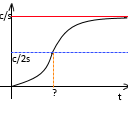
\includegraphics{resources/nonLinearDifferencialEquation_HumanGrow.png}

  其中$\cfrac{c}{s}$称为稳态,到了这里就会保持稳定,不会改变了.不过其实到不了哪里,只会一直接近而已.这就是这个式子所代表的人口曲线了.

  那么就是解方程的环节了.有很多方法,先试试一个好使的:尝试$y = \cfrac{1}{P}$.然后尝试把整个方程写成y的形式.这是解这个方程的技巧,而解非线性方程常常需要一些技巧.

  看看这个方程长啥样子:$\cfrac{dy}{dt} = -\cfrac{\cfrac{dP}{dt}}{P^2}$而$\cfrac{dP}{dt}$是已知的,所以将他代进来,得到$-\cfrac{cP - sP^2}{P^2}$.将负号写进去,得到一个s:$s - \cfrac{c}{P}$.查看前面的推导能发现:$\cfrac{1}{p} = y$.所以得到$s - cy$.于是$\cfrac{dy}{dt}$变成了线性的,它还含有资源项s,而增长率项还含有一个-c.也许仔细想想为什么

  那么写出y的解:$y(t) - \cfrac{s}{c} = (y(0) - \cfrac{s}{c})e^{-ct}$这就是y的解.$y = \cfrac{1}{P}$,接下来就是要回代了:

  $\cfrac{1}{P(t)} - \cfrac{s}{c} = (\cfrac{1}{P(0)} - \cfrac{s}{c})e^{-ct}$,接下来的一堆化简就不写了.

  这种模型称为logistic方程(只是为了提一下)

  接下来再来一个有意思的方程:捕食者与猎物的方程:

  这里有两个未知数:猎物——记作$v$,捕食者——记作$u$,表示的都是两者的总数.如果猎物不够,捕食者就会减少.捕食者减少,猎物就会增加.因此这里有正的$u \cdot v$

  这是公式:

  前面有个$-cu$,表示没有食物的情况,捕食者将会慢慢灭绝.

  但如果猎物存在,那么资源项就会正比于$uv$.

  所以$\cfrac{du}{dt} = -cu + suv$

  那么$\cfrac{dv}{dt}$呢?情况大不相同.他们被捕食,因此有$-Suv$,同时也有正的增长率$Cv$

  那么这就是一个模型了.剧透一下:这玩意叫偏微分方程(Partical Differential Equation),简称PDE,他比常微分方程(Ordinary Differential Equation, ODE)包含了更多的信息.也更难解.

}%关于增长的微分方程结尾

}%微分方程结尾

}%微积分结尾

\section{多元微积分}{
  注:如果忘了什么是偏导数就去上一章回顾.
  %# TODO: 重新学一遍

  \subsection{隐函数}{

    \subsubsection{隐函数存在定理}{

    }%隐函数存在定理结尾

  }%隐函数结尾

 }%多元微积分结尾

\section{高等代数/线性代数}{

 }%高等代数/线性代数结尾

\section{数论}{

 }%数论结尾

\section{场论}{

  \subsection{场论基本内容}{
    注:矢量 = 向量,有时候会混着用,一般是那个顺口用哪个.

    \subsubsection{矢量函数/向量函数}{
      向量值函数,有时也称为向量函数,是一个单变量或多变量的、值域是多维向量或者无穷维向量的集合的函数.向量值函数的输入可以是一个标量或者一个向量(定义域的维度可以是1或大于1);定义域的维度不取决于值域的维度.

      即:设有数性变量t和变矢量$\vec{A}$.若对于t在某个范围内的每一个数值,$\vec{A}$都有一个确定的矢量和它对应,则称$\vec{A}$为数性变量t的矢量函数.记为:$\vec{A} = A(t)$,也可以写作$\vec{A} = A_x(t)i + A_y(t)j + A_z(t)k$

      矢量函数$A(t)$的起点取在坐标原点,其终点随变量t变化描绘出了一条曲线,该曲线叫做$A(t)$的矢端曲线.也就是$A(t)$的图像.
    }%矢量函数/向量函数结尾

    \subsubsection{矢量向量函数的极限}{
      用$\delta-\epsilon$语言来说:

      设矢量函数$A(t)$在点$t_0$的某个邻域内有定义(在$t_0$点可以没有),$\vec{A}_0$为常矢量.若对于任意给定$\epsilon > 0$,都存在一个$\delta > 0$,当$0 < |t - t_0| < \delta$时,就有$|A(t) - \vec{A}_0|$成立,则称当$t \to t_0$时,$A(t)$有极限$\vec{A}_0$,记作:

      \begin{center}
        $\limNormal{t \to t_0}A(t) = \vec{A}_0$
      \end{center}

      注:在直角坐标系中有:

      \begin{center}
        $\limNormal{t \to t_0}A_x(t) = A_{0x}$ \\
        $\limNormal{t \to t_0}A_y(t) = A_{0y}$ \\
        $\limNormal{t \to t_0}A_z(t) = A_{0z}$
      \end{center}

      其中$\vec{A}_0 = A_{0x}\vec{i} + A_{0y}\vec{j} + A_{0z}\vec{k}$
    }%矢量函数的极限结尾

    \subsubsection{矢量函数的连续}{
      设$A(t)$在$t_0$的某领域内有定义,且 :

      \begin{center}
        $\limNormal{t \to t_0}A(t) = A(t_0)$
      \end{center}

      即 :

      \begin{center}
        $\limNormal{t \to t_0}A_x(t) = A_x(t_0)$ \\
        $\limNormal{t \to t_0}A_y(t) = A_y(t_0)$ \\
        $\limNormal{t \to t_0}A_y(t) = A_y(t_0)$
      \end{center}

      就称$A(t)$在$t_0$点连续.
    }%矢量函数的连续结尾

    \subsubsection{矢量函数的导数}{
      设矢量函数$A(t)$在点t处有增量$\Delta A = A(t + \Delta t) - A(t)$

      当$\Delta t \to 0$时,$\cfrac{\Delta A}{\Delta t} = \cfrac{A(t + \Delta t) - A(t)}{\Delta t}$的极限存在,则称此极限值为$A(t)$在点t处的导向量/导矢.即 :

      \begin{center}
        $A\derivative(t) = \cfrac{dA(t)}{dt} = \limNormal{\Delta t \to 0}\cfrac{\Delta A}{\Delta t} = \limNormal{\Delta t \to 0}\cfrac{A(t + \Delta t) - A(t)}{\Delta t}$
      \end{center}

      以下为导数公式 :

      \begin{itemize}
        \item $\cfrac{d}{dt}(\vec{\mathConstant}) = 0$ ($\vec{\mathConstant}$为常矢量)
        \item $\cfrac{d}{dt}(\vec{A} \pm \vec{B}) = \cfrac{d}{dt}\vec{A} \pm \cfrac{d}{dt}\vec{B}$
        \item $\cfrac{d}{dt}(u\vec{A}) = \cfrac{du}{dt}\vec{A} + u\cfrac{d\vec{A}}{dt}$\ 当u是常数k时,$\cfrac{d}{dt}(kA) = k\cfrac{d\vec{A}}{dt}$
        \item $\cfrac{d}{dt}(\vec{A}\cdot\vec{B}) = \vec{A}\cdot\cfrac{d\vec{B}}{dt} + \vec{B}\cdot\cfrac{d\vec{A}}{dt}$
        \item $\cfrac{d}{dt}(\vec{A}\times\vec{B}) = \vec{A}\times\cfrac{d\vec{B}}{dt} + \vec{B}\times\cfrac{d\vec{A}}{dt}$
        \item 若$\vec{A} = A(u),u = u(t)$,则$\cfrac{d\vec{A}}{dt} = \cfrac{d\vec{A}}{du}\cdot\cfrac{du}{dt}$
      \end{itemize}

      这些公式与函数的导数公式类似.只是在乘法上向量有点乘和叉乘两种乘法,而且没有除法,所以没有除法法则.

      向量导数在几何上的直观图像为:

      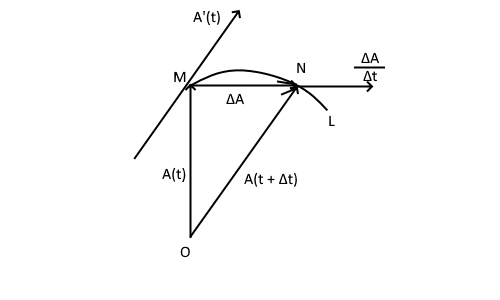
\includegraphics{resources/derivativeOfVectorFunction.png}

      即 : 矢径长度随时间的变化率
    }%矢量函数的导数

    \subsubsection{矢量函数的微分}{
      称$dA(t) = A\derivative(t)dt\ (\Delta t = dt)$为$A(t)$在$t$处的微分.在直角坐标系中有:

      $\cfrac{d\vec{A}}{dt} = A\derivative_x(t)\vec{i} + A\derivative_y(t)\vec{j} + A\derivative_z(t)\vec{k}$

      即 :

      $d\vec{A} = dA_x(t)\vec{i} + dA_y(t)\vec{j} + dA_z(t)\vec{k} = (A\derivative_x(t)\vec{i} + A\derivative_y(t)\vec{j} + A\derivative_z(t)\vec{k})dt$
    }%矢量函数的微分结尾

    \subsubsection{矢量函数的不定积分}{
      若$A\derivative(t) = a(t)$,则称$A(t)$是$a(t)$的原函数.$a(t)$的原函数的一般形式叫做$a(t)$的不定积分,记作 :

      $\int a(t)dt$

      若$A\derivative(t)$是$a(t)$的一个原函数,则有 :

      $\int a(t)dt = A(t) + \vec{\mathConstant}$\qquad ($\vec{\mathConstant}$为任意常矢)
    }

    \subsubsection{矢量函数的定积分}{
      类似于数性函数,$a(t)$在$[t_1,t_2]$上的定积分的定义为 :

      $\definiteIntegral{t_2}{t_1}a(t)dt = \limNormal{n \to \infty}\limNormal{\lambda \to 0}\upDownSum{n}{i = 1}a(\xi_i)\Delta t_i$

      若$A(t)$是$a(t)$的一个原函数,则有 :
      $$
        \definiteIntegral{t_2}{t_1}a(t)dt = A(t_2) - A(t_1)\qquad \mbox{(微积分基本定理)}
      $$
      在直角坐标系中可分解为 :
      $$
        \definiteIntegral{t_2}{t_1}a(t)dt = \definiteIntegral{t_2}{t_1}a_x(t)dt\vec{i} + \definiteIntegral{t_2}{t_1}a_y(t)dt\vec{j} + \definiteIntegral{t_2}{t_1}a_z(t)dt\vec{k}
      $$
    }%矢量函数的定积分

    \begin{itemize}
      \item 从上述内容看出,矢量函数的微积分与数学分析(高等数学)中的微积分相类似,不过矢量函数要复杂些,他在直角坐标系中分解成三个数性函数,即他的三个分量.对矢量函数进行某一种运算,也就等于对他的各个分量进行这种运算.
      \item 矢量分解与坐标选取有关.在不同的坐标系中,有不同的表现形式,有的可能复杂的多.这里主要讨论直角坐标系的分解问题,多数问题还是会用分量表示.
    \end{itemize}

  }%场论基本内容结尾

  \subsection{场的分类与表示法}{

    \subsubsection{场的概念}{
      某一物理量在空间的分布就称为"场".在这个空间发生了物理现象,也就有物理量在这个空间分布.
    }%场的概念结尾

    \subsubsection{场的分类与表示}{
      场中每一点$M:(x,y,z)$都对应着一个物理量,即某个函数$\defFunction{M}$,如果这个函数是数量值函数,这种场就叫做数量场.如果是向量值函数,那么这种场就叫做矢量场.

      场中的物理量往往与点的位置有关,而且还将随时间变化.会随时间变化的场就叫做不稳定场(或不定常场),表示为 :
      $$
        u= \defFunction{M,t},\vec{A} = A(M,t)
      $$
      在三维直角坐标系(可推广至任意维)下也可分解为 :
      $$
        u = \defFunction{x,y,z,t}
      $$
      $$
        \vec{A} = A(x,y,z,t) = A_x(x,y,z,t)\vec{i} + A_y(x,y,z,t)\vec{j} + A_z(x,y,z,t)\vec{k}
      $$\spaceline

      如果场中物理量不随时间变换,这种场叫做稳定场(定常场),表示为 :
      $$
        u= \defFunction{M}\qquad \vec{A} = A(M)
      $$
      在三维直角坐标系(可推广)下也可以分解为 :
      $$
        u= \defFunction{x,y,z}
      $$
      $$
        \vec{A} = A(x,y,z) = A_x(x,y,z)\vec{i} + A_y(x,y,z)\vec{j} + A_z(x,y,z)\vec{k}
      $$
      在不稳定场中,美以固定时刻也就是稳定场.在场论中,讨论稳定场是基础.对于不稳定场,可以在讨论不稳定场的基础上再讨论对时间的变化.因此接下来一大段着重讨论稳定场的规律.
    }%场的分类与表示

    \subsubsection{场的直观表示}{
      在数量场中,物理量是点的坐标$(x,y,z)$的函数 :
      $$
        u = \defFunction{x,y,z}
      $$
      当u为某常数$\mathConstant$时,所有满足$\defFunction{x,y,z} = \mathConstant$的点就组成一个曲面.这个曲面的特点是在其上的点$(x,y,z)$处的函数值$u$相等,即
      $$
        \defFunction{x,y,z} = \mathConstant
      $$
      此曲面称为等值面,在平面中也被称为等值线.

      在矢量场中用矢量线表示.场中的曲线$L$,若他每点的切线方向与场在该点的矢量方向平行,则$L$称为该矢量场的矢量线.矢量线满足微分方程 :
      $$
        \cfrac{dx}{A_x} = \cfrac{dy}{A_y} = \cfrac{dz}{A_z}
      $$

      \begin{itemize}
        \item 矢量线$L$不止有一个,而是一族曲线.矢量线$L$存在于场中,$L$上每一点都有一个矢量$\vec{A} = \begin{bmatrix}
                  A_x & A_y & A_z
                \end{bmatrix}$
        \item 矢量线$L$只反映矢量场在$L$上每点的方向,并没有大小数量关系.
        \item 等值面(线)是满足等函数值的自变量全体.因为C时任意常数,所以$\defFunction{x,y,z} = \mathConstant$表示等值面族.
      \end{itemize}
    }%场的直观表示结尾

  }%场的分类与表示法结尾

  \subsection{方向导数与梯度}{

    \subsubsection{方向导数的定义}{
      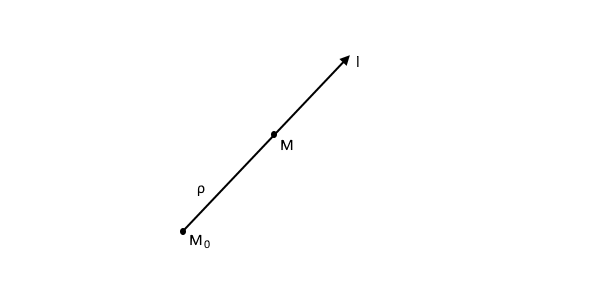
\includegraphics{resources/directionDerivative1.png}

      从数量场$u= u(M)$中任一点$M_0$出发引一条有向射线$l$,在$l$上任取一点$M$,记$M_0M = \rho$,当沿$l$,$M \to M_0$时,此式的极限存在 :
      $$
        \cfrac{\Delta u}{\rho} = \cfrac{u(M) - u(M_0)}{M_0M}
      $$
      称此极限值为函数$u(M)$在点$M_0$处沿方向$l$的方向导数,记为$\directionDerivative{u}{l}{M_0}$,即 :
      $$
        \directionDerivative{u}{l}{M_0} = \limNormal{M \to M_0}\cfrac{u(M) - u(M_0)}{M_0M}
      $$

      \begin{itemize}
        \item 方向导数是一个数量,他与点$M_0$有关,也与方向$l$有关.
        \item {
              以平面数量场为例说明方向导数的意义 :

              设数量场
              $$
                u = \defFunction{x,y}
              $$
              不难看出 :
              % #TODO 画图
              $$
                \cfrac{\Delta u}{\rho} = \cfrac{u(M) - u(M_0)}{M_0M} = \cfrac{\defFunction{M} - \defFunction{M_0}}{M_0M}
              $$
              正是沿着$l$方向,函数$\defFunction{x,y}$从点$M_0$到点$M$的平均升高,即平均变化率.而极限 :
              $$
                \limNormal{M \to M_0}\cfrac{\Delta u}{\rho} = \limNormal{M \to M_0}\cfrac{\defFunction{M} - \defFunction{M_0}}{M_0M} (\mbox{沿着}l)
              $$
              是$u = \defFunction{x,y}$在点$M_0$沿$l$的变化率.所以方向导数是变化率,它反映了函数$u = \defFunction{x,y}$在$l$方向上的增减情况.当$\directionDerivative{u}{l}{M_0} > 0$,表示函数$u = \defFunction{x,y}$在点$M_0$沿方向$l$是增加的,越大表示增加的越快.反之亦然.
              }
        \item 偏导数是方向导数的特例.比如当$l$指向x轴正向时,$\cfrac{\partial u}{\partial l} = \cfrac{\partial u}{\partial x}$,当$l$指向y轴正向时,$\cfrac{\partial u}{\partial l} = \cfrac{\partial u}{\partial y}$.
        \item 有时候要考虑函数沿某曲线C的导数.函数沿曲线C的每一点的切线方向的方向导数叫做函数沿曲线C的导数.
      \end{itemize}
    }%方向导数的定义结尾

    \subsubsection{方向导数的计算公式}{
      设$u= u(x,y,z)$在$M_0(x_0,y_0,z_0)$处可微,l的方向余弦时$\cos\alpha,\cos\beta,\cos\gamma$,则u在点$M_0$沿$l$的方向导数为 :
      $$
        \directionDerivative{u}{l}{M_0} = \directionDerivative{u}{x}{M_0}\cos\alpha + \directionDerivative{u}{y}{M_0}\cos\beta + \directionDerivative{u}{z}{M_0}\cos\gamma
      $$
      或者 :
      $$
        \directionDerivative{u}{l}{M_0} = \partialDerivativeFrac{u}{x}\cos\alpha + \partialDerivativeFrac{u}{y}\cos\beta + \partialDerivativeFrac{u}{z}\cos\gamma
      $$
    }%方向导数的计算公式结尾    

    \subsubsection{梯度}{
      设数量场$u = u(M)$,如果在场中任一点$M$处,存在非零矢量$\vec{G}$,其方向为函数$u(M)$在$M$点处方向导数的最大的方向,其模$|\vec{G}|$这个最大的方向导数值,则称矢量$\vec{G}$为数量场$u$在点$M$处的梯度,记为 :
      $$
        grad\ u = \vec{G}
      $$
      在直角坐标系中有 :
      $$
        grad\ u = \begin{bmatrix}
          \partialDerivativeFrac{u}{x} & \partialDerivativeFrac{u}{y} & \partialDerivativeFrac{u}{z}
        \end{bmatrix} = \partialDerivativeFrac{u}{x}\vec{i} + \partialDerivativeFrac{u}{y}\vec{j} + \partialDerivativeFrac{u}{z}\vec{k}
      $$

      引入$grad\ u = \triangledown u$

      \begin{itemize}
        \item 梯度是刻划数量场的概念.数量场的梯度是一个矢量.
        \item 任一点的梯度垂直于过该点的等值面(线),并且指向$u(M)$增大的一方.因而梯度方向平行于等值面(线)的法线方向.
        \item 数量场的每一点都有一个梯度,他是矢量,数量场的梯度场是矢量场,称为$u(M)$的梯度场.
        \item $\partialDerivativeFrac{u}{l} = \triangledown u \cdot l_0$,其中$l_0= \cfrac{l}{|l|}$
        \item $\triangledown$称为$\triangledown$算子
      \end{itemize}
    }%梯度结尾

    \subsubsection{梯度的运算公式}{
      \begin{itemize}
        \item $\triangledown \mathConstant = 0$
        \item $\triangledown (\mathConstant u) = \mathConstant \triangledown u$
        \item $\triangledown (u \pm v) = \triangledown u + \triangledown v$
        \item $\triangledown (uv) = v\triangledown u + u\triangledown v$
        \item $\triangledown (\cfrac{u}{v}) = \cfrac{v\triangledown u - u\triangledown v}{v^2}\qquad (v \neq 0)$(注意:与导数的顺序不同)
        \item $\triangledown \defFunction{u} = \fDerivative{u}\triangledown u$
      \end{itemize}
    }%梯度的运算公式

  }%方向导数与梯度结尾

 }%场论结尾

\section{群论}{

 }%群论结尾

\section{矩阵论}{

 }%矩阵论结尾

 \section{离散数学}{
   
 }%离散数学结尾

}%数学篇结尾

\chapter{计算机科学}{

  \section{编程}{


   }%编程结尾

  \section{网络安全}{


   }%网络安全结尾

  \section{计算机图形学}{
    注:本章中向量默认为列向量.

    \subsection{对于线性代数部分的补充与扩展}{

      在计算机图形学中线性代数的主要作用是操纵与计算空间中对象的变化.由此衍生出了一些特殊的东西.

      同时有一部分重要的常用基础内容放在了数学篇中的空间解析几何部分.

      \begin{enumerate}
        \item {向量叉乘的对偶矩阵:
              $$\vec{a} \times \vec{b}
                =
                \begin{bmatrix}
                  y_az_b - y_bz_a \\
                  z_ax_b - x_az_b \\
                  x_ay_b - y_ax_b
                \end{bmatrix}
                =
                A * \vec{b}
                =
                \begin{bmatrix}
                  0    & -z_a & y_a  \\
                  z_a  & 0    & -x_a \\
                  -y_a & x_a  & 0
                \end{bmatrix}
                \begin{bmatrix}
                  x_b \\
                  y_b \\
                  z_b
                \end{bmatrix}
              $$
              }
        \item 非满秩矩阵意味着将空间变换到了更低的维度.
        \item 特征向量是指在进行了矩阵所代表的线性变换后方向没改变向量,特征值则是指特征向量的缩放倍数.
        \item 逆矩阵所代表的变换成为逆变换,是原矩阵所代表的变换的反向操作,一个矩阵乘以他的逆矩阵是单位阵,这从几何上的直观理解就是什么都没做,两次操作互相抵消了.
      \end{enumerate}
    }

    \subsection{变换}{
      变换按照作用对象可以分为:
      \begin{enumerate}
        \item Modeling 模型变换
        \item Viewing 视角变换
      \end{enumerate}

      按照作用效果可以分为:
      \begin{enumerate}
        \item scale 缩放变换
        \item rotate 旋转变换
        \item shear 剪切变换
      \end{enumerate}

      如同3b1b的观点,将目标空间看作矩阵的列空间.而矩阵每一列都对应了列空间中的一个基向量,拿2维空间举例:
      $$
        \begin{bmatrix}
          1 & 0 \\
          0 & 1
        \end{bmatrix}
      $$

      假设第一列代表了$x$轴的单位向量$i$,则第二列代表了$y$轴的单位向量$j$

      因此,对矩阵进行操作就相当于对矩阵所代表的空间进行操作.

      例如:$$
        \begin{bmatrix}
          2 & 1 \\
          1 & 2
        \end{bmatrix}
      $$

      这个矩阵就代表着将单位向量$i$移动到了坐标$(2,1)$,将单位向量$j$移动到了坐标$(1,2)$.整个二维空间都是由这两个单位向量所张成的.随着单位向量的移动,整个空间也就随之而变形.这种操作被称为变换.
      其中一类最简单的变换称为线性变换,在线性代数篇中已有了详细解释.

      旋转矩阵的表示原理如下:

      先看看二维:

      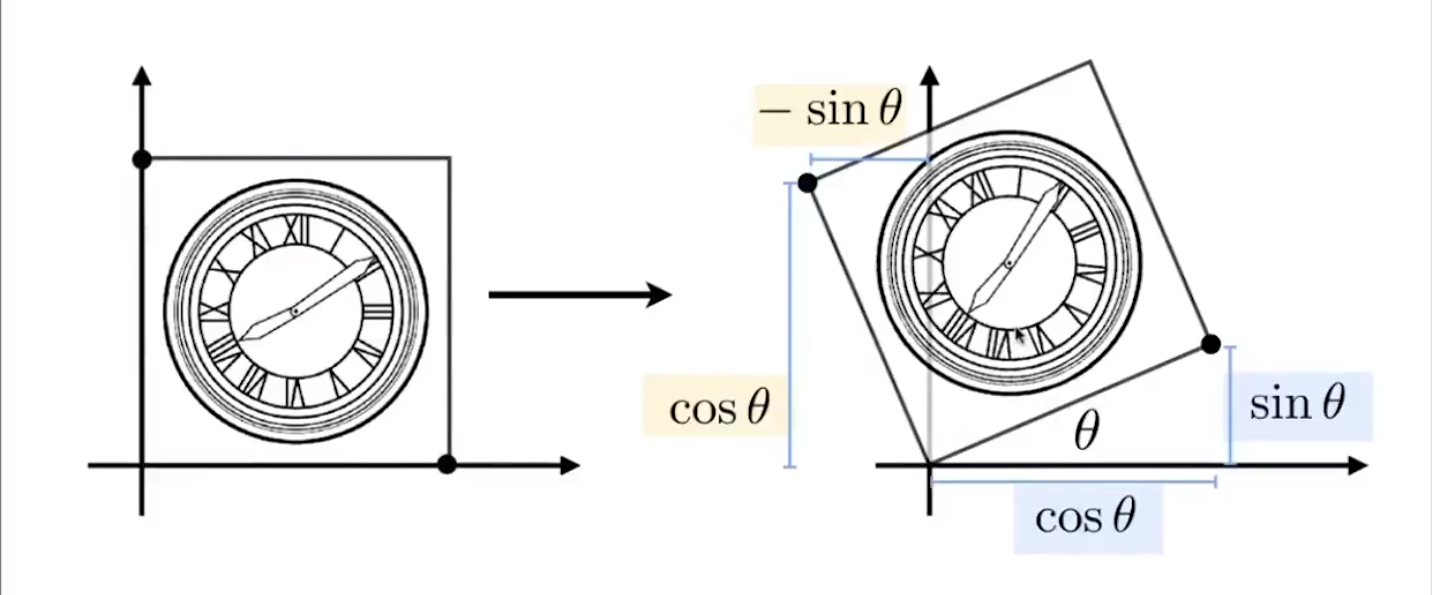
\includegraphics[scale=0.25]{resources/rotateMatrixGraphics.png}

      因此二维的旋转矩阵$$
        R_\theta = \begin{bmatrix}
          \cos\theta & -\sin\theta \\
          \sin\theta & \cos\theta
        \end{bmatrix}
      $$


      \subsubsection{齐次坐标}{
        由于单纯的线性变换并不能让对象动起来,依然只能在原点操作,所以需要齐次坐标表示空间上的位移.

        如下图:

        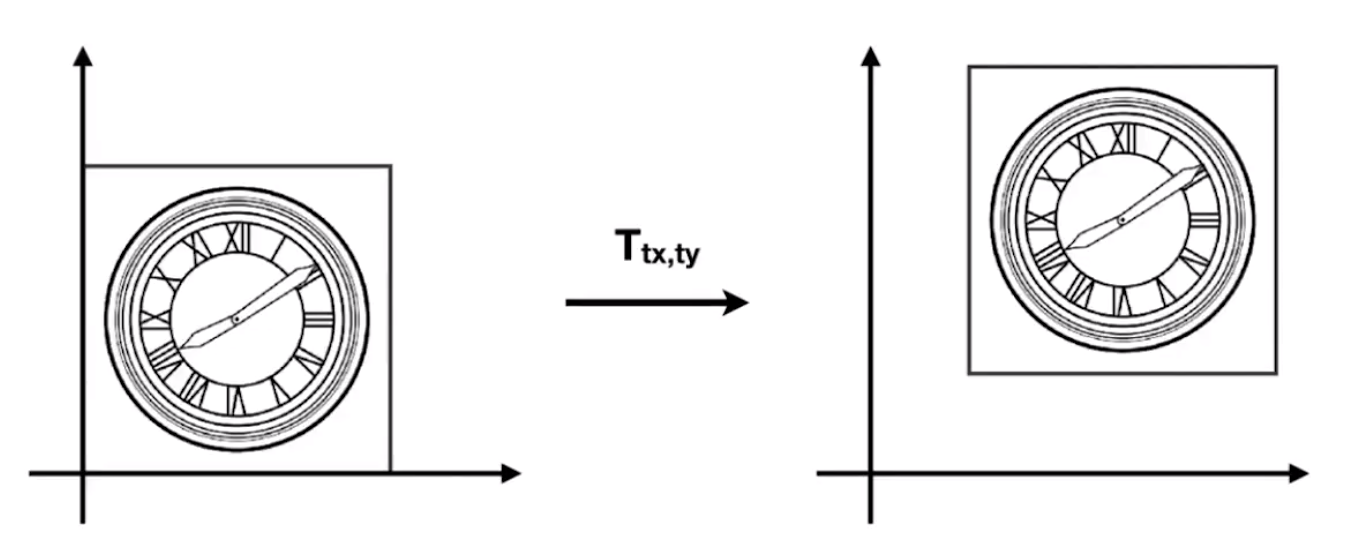
\includegraphics[scale=0.25]{resources/homogeneous_coordinates.png}

        用$x\prime$和$y\prime$来表示变换后的坐标,公式为:

        $x\prime = x + t_x$

        $y\prime = y + t_y$

        仔细思考一下发现似乎并不能写成矩阵$A\vec{x} = \vec{b}$的形式.

        事实上应该写成这样:
        $$
          \begin{bmatrix}
            x\prime \\
            y\prime
          \end{bmatrix}
          =
          \begin{bmatrix}
            a & b \\
            c & d
          \end{bmatrix}
          \begin{bmatrix}
            x \\
            y
          \end{bmatrix}
          +
          \begin{bmatrix}
            t_x \\
            t_y
          \end{bmatrix}
        $$

        因此平移变换不属于线性变换.但是人们不想要特殊情况,于是引入了齐次坐标:

        还是拿二维的情况举例,增加一个维度,将二维的点表示为:
        $$\begin{bmatrix}
            x & y & 1
          \end{bmatrix}^T$$

        将二维向量表示为:
        $$\begin{bmatrix}
            x & y & 0
          \end{bmatrix}^T$$

        也就是说:再多增加一个维度用于说明表示的是一个点还是一个向量,这是因为向量具有平移不变性,不管怎么移动表示的始终是一个方向.

        齐次坐标的好处就在这里,它是这么用的:

        $$\begin{bmatrix}
            x\prime \\
            y\prime \\
            w\prime
          \end{bmatrix}
          =
          \begin{bmatrix}
            1 & 0 & t_x \\
            0 & 1 & t_y \\
            0 & 0 & 1
          \end{bmatrix}
          \cdot
          \begin{bmatrix}
            x \\
            y \\
            1
          \end{bmatrix}
          =
          \begin{bmatrix}
            x + t_x \\
            y + t_y \\
            1
          \end{bmatrix}
        $$

        更直观一点:可以这么理解:
        \begin{itemize}
          \item 向量 + 向量 = 向量, 向量相加还是向量 $0 + 0 = 0$
          \item 点 - 点 = 向量, 两点相减得到向量 $1 - 1 = 0$
          \item 点 + 向量 = 点, 一个点加一个向量结果是一个点 $0 + 1 = 1$
          \item 点 + 点 = 两个点的中点, $1 + 1 = 2$,原因见扩充定义.
        \end{itemize}
        扩充定义如下:
        $$\begin{bmatrix}
            x \\
            y \\
            w
          \end{bmatrix} = \begin{bmatrix}
            x \\
            y \\
            w
          \end{bmatrix}\cdot\cfrac{1}{w} = \begin{bmatrix}
            \cfrac{x}{w} \\
            \cfrac{y}{w} \\
            1
          \end{bmatrix}$$

        {\bfseries于是总结,给出以下下定义:}\\\\\indent
        仿射变换(Affine transformation) = 线性变换(Linear transformation) + 位移(transformation)

        即:
        $$\begin{bmatrix}
            x\prime \\
            y\prime
          \end{bmatrix}
          =
          \begin{bmatrix}
            a & b \\
            c & d
          \end{bmatrix}
          \cdot
          \begin{bmatrix}
            x \\
            y
          \end{bmatrix}
          +
          \begin{bmatrix}
            t_x \\
            t_y
          \end{bmatrix}$$

        都可以写成齐次坐标(homogeneous coordinates)的形式

        即:
        $$\begin{bmatrix}
            x\prime \\
            y\prime \\
            1
          \end{bmatrix}
          =
          \begin{bmatrix}
            a & b & t_x \\
            c & d & t_y \\
            0 & 0 & 1
          \end{bmatrix}
          \cdot
          \begin{bmatrix}
            x \\
            y \\
            1
          \end{bmatrix}$$

        {\bfseries不如直接将其他操作的齐次坐标形式补全吧?}
        \begin{itemize}
          \item 缩放(scale) : $$S(s_x, s_y) = \begin{bmatrix}
                    s_x & 0   & 0 \\
                    0   & s_y & 0 \\
                    0   & 0   & 0
                  \end{bmatrix}$$
          \item 旋转(rotation) : $$R(\alpha) = \begin{bmatrix}
                    \cos\alpha & -\sin\alpha & 0 \\
                    \sin\alpha & \cos\alpha  & 0 \\
                    0          & 0           & 1
                  \end{bmatrix}$$
          \item 平移(translation) : $$T(t_x, t_y) = \begin{bmatrix}
                    1 & 0 & t_x \\
                    0 & 1 & t_y \\
                    0 & 0 & 1
                  \end{bmatrix}$$
        \end{itemize}

      }%齐次坐标结尾

      \subsubsection{组合变换}{
        可以通过组合各个基础变换以形成复杂的变换效果.

        组合方法为对应矩阵按照顺序从右向左做乘法.

        大部分时候组合顺序至关重要.

      }%组合变换结尾

      \subsubsection{三维变换}{
        以上结论都可以用于三维,推而广之:\\

        齐次坐标:\begin{itemize}
          \item 三维点:$$\begin{bmatrix}
                    x \\
                    y \\
                    z \\
                    1
                  \end{bmatrix}$$
          \item 三维向量:$$\begin{bmatrix}
                    x \\
                    y \\
                    z \\
                    0
                  \end{bmatrix}$$
        \end{itemize}

        $\left[x\ y\ z\ w\right]^T$,当$w$不等于$1$他所表示的三维的点其实是(第四个维度已略去):
        $$\begin{bmatrix}
            \cfrac{x}{w} \\
            \cfrac{y}{w} \\
            \cfrac{z}{w} \\
          \end{bmatrix}$$

        同样的,三维空间中齐次坐标描述的仿射变换的矩阵是$4 \times 4$的:
        $$\begin{bmatrix}
            x\prime \\
            y\prime \\
            z\prime \\
            1
          \end{bmatrix}
          =
          \begin{bmatrix}
            a & b & c & t_x \\
            d & e & f & t_y \\
            g & h & i & t_z \\
            0 & 0 & 0 & 1
          \end{bmatrix}
          \cdot
          \begin{bmatrix}
            x \\
            y \\
            z \\
            1
          \end{bmatrix}$$

        将二维操作类比过来:

        \begin{itemize}
          \item 缩放 : $$
                  S(s_x,s_y,s_z) =\begin{bmatrix}
                    s_x & 0   & 0   & 0 \\
                    0   & s_y & 0   & 0 \\
                    0   & 0   & s_z & 0 \\
                    0   & 0   & 0   & 1
                  \end{bmatrix}
                $$
          \item 平移 : $$
                  T(t_x,t_y,t_z) = \begin{bmatrix}
                    1 & 0 & 0 & t_x \\
                    0 & 1 & 0 & t_y \\
                    0 & 0 & 1 & t_z \\
                    0 & 0 & 0 & 1
                  \end{bmatrix}
                $$
          \item 三维旋转(绕某个轴逆时针旋转) :
                $$
                  R_x(\alpha) = \begin{bmatrix}
                    1 & 0          & 0           & 0 \\
                    0 & \cos\alpha & -\sin\alpha & 0 \\
                    0 & \sin\alpha & \cos\alpha  & 0 \\
                    0 & 0          & 0           & 1
                  \end{bmatrix}
                $$

                $$
                  R_y(\alpha) = \begin{bmatrix}
                    \cos\alpha  & 0 & \sin\alpha & 0 \\
                    0           & 1 & 0          & 0 \\
                    -\sin\alpha & 0 & \cos\alpha & 0 \\
                    0           & 0 & 0          & 1
                  \end{bmatrix}
                $$

                $$
                  R_z(\alpha) = \begin{bmatrix}
                    \cos\alpha & -\sin\alpha & 0 & 0 \\
                    \sin\alpha & \cos\alpha  & 0 & 0 \\
                    0          & 0           & 1 & 0 \\
                    0          & 0           & 0 & 1
                  \end{bmatrix}
                $$
          \item 三维旋转(欧拉角) : $R_{xyz}(\alpha,\beta,\gamma) = R_x(\alpha)R_y(\beta)R_z(\gamma)$
          \item 三维旋转($\vec{I}$绕任意轴n旋转角度$\alpha$)(罗德里格斯旋转公式) : $$
                  R(n,\alpha) = \cos(\alpha)\vec{I} + (1 - \cos(\alpha))\vec{n}\vec{n}\transpose + \sin(\alpha)\begin{bmatrix}
                    0    & -n_z & n_y  \\
                    n_z  & 0    & -n_x \\
                    -n_y & n_x  & 0
                  \end{bmatrix}
                $$
                (其中$\vec{n}$为旋转轴的单位向量)
        \end{itemize}
      }%三维变换结尾

      \subsubsection{观测变换}{
        一般来说拍一张照片的步骤如下 :

        \begin{enumerate}
          \item 找到一个好的位置摆放人物(模型变换,model transformation)
          \item 找到一个好的"角度"来放下相机(视图变换,view transformation)
          \item 按下快门(投影变换,projection transformation)
        \end{enumerate}

        \begin{itemize}
          \item {
                视图变换(view transformation) :

                首先定义相机:
                \begin{itemize}
                  \item 位置(Position) : $\vec{e}$
                  \item 视线方向(Look-at/gaze direction) : $\hat{\vec{g}}$
                  \item 向上方向(UP direction) : $\hat{\vec{t}}$ (注:这个表示的是相机自身的旋转,此向量垂直于上面两个向量张成的平面)
                \end{itemize}

                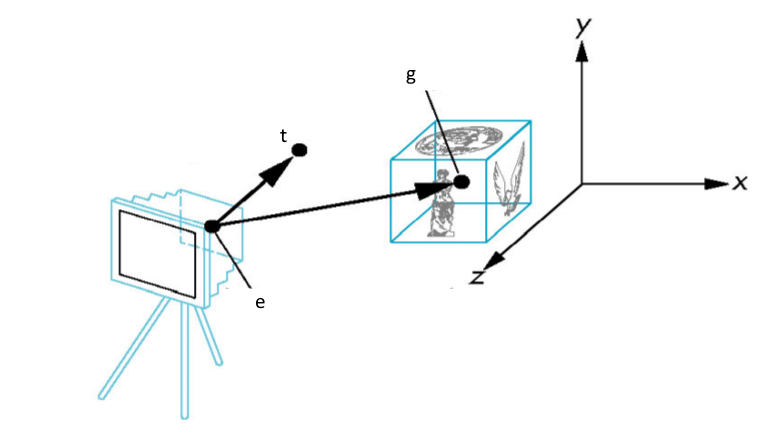
\includegraphics[scale=0.9]{resources/viewTransformation.png}

                值得注意的是: 定义相机永远在原点,视线朝向-z方向,以y轴作为向上方向(约定俗成,这么做有很多好处)

                所以在实际情况中,需要将相机和被观测的对象视作一个整体,进行如下操作:
                \begin{enumerate}
                  \item 将$\vec{e}$平移到原点.
                  \item 将$\hat{\vec{g}}$旋转到-z方向
                  \item 将$\hat{\vec{t}}$旋转到y方向
                  \item 将$\hat{\vec{g}} \times \hat{\vec{t}}$旋转到x方向
                \end{enumerate}

                这一系列的矩阵操作记作$M_{view}$,如下:

                \begin{itemize}
                  \item 令$M_{view} = R_{view}T_{view}$
                  \item 将$\vec{e}$平移到原点 : $$
                          T_{view} = \begin{bmatrix}
                            1 & 0 & 0 & -x_e \\
                            0 & 1 & 0 & -y_e \\
                            0 & 0 & 1 & -z_e \\
                            0 & 0 & 0 & 1
                          \end{bmatrix}
                        $$
                  \item 将$\hat{\vec{g}}$旋转到-z方向,将$\hat{\vec{t}}$旋转到y方向,($\hat{\vec{g}} \times \hat{\vec{t}}$)旋转到x方向 : $$
                          R_{view} = \begin{bmatrix}
                            x_{\hat{\vec{g}} \times \hat{\vec{t}}} & y_{\hat{\vec{g}} \times \hat{\vec{t}}} & z_{\hat{\vec{g}} \times \hat{\vec{t}}} & 0 \\
                            x_{\hat{\vec{t}}}                      & y_{\hat{\vec{t}}}                      & z_{\hat{\vec{t}}}                      & 0 \\
                            x_{-\hat{\vec{g}}}                     & y_{-\hat{\vec{g}}}                     & z_{-\hat{\vec{g}}}                     & 0 \\
                            0                                      & 0                                      & 0                                      & 1
                          \end{bmatrix}
                        $$
                  \item 仔细思考,发现上面想要直接计算出来过于繁琐,应当反向思考—求出将坐标系变换到相机的位置的矩阵再求逆 : $$
                          R^{-1}_{view} = \begin{bmatrix}
                            x_{\hat{\vec{g}} \times \hat{\vec{t}}} & x_{\hat{\vec{t}}} & x_{-\hat{\vec{g}}} & 0 \\
                            y_{\hat{\vec{g}} \times \hat{\vec{t}}} & y_{\hat{\vec{t}}} & y_{-\hat{\vec{g}}} & 0 \\
                            z_{\hat{\vec{g}} \times \hat{\vec{t}}} & z_{\hat{\vec{t}}} & z_{-\hat{\vec{g}}} & 0 \\
                            0                                      & 0                 & 0                  & 1
                          \end{bmatrix}
                        $$
                        由于旋转矩阵是正交矩阵,所以求逆等于求转置.
                \end{itemize}
                随着相机的变换,其他所有物体也应当跟着变换,这样才能保证拍出来的是同样的照片.
                }

          \item {
                投影变换(projection transformation) :

                投影分为两种 : 正交投影(Perspective projection)和透视投影(Orthographic projection):

                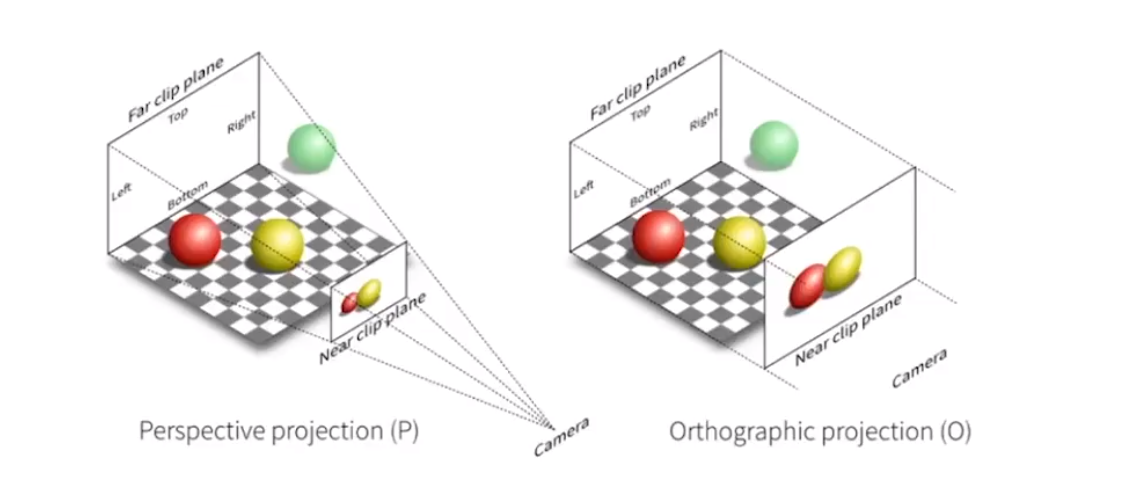
\includegraphics[scale=0.5]{resources/twoProjectionTransformation.png}

                两种投影的本质区别就在于是否有近大远小的现象.

                \begin{itemize}
                  \item {
                        正交投影(Orthographic projection) :

                        先定义一个空间中的立方体, 给出三个轴的范围$[l,r]\times[b,t]\times[f,n]$,平移并缩放到标准立方体$[-1,1]^3$

                        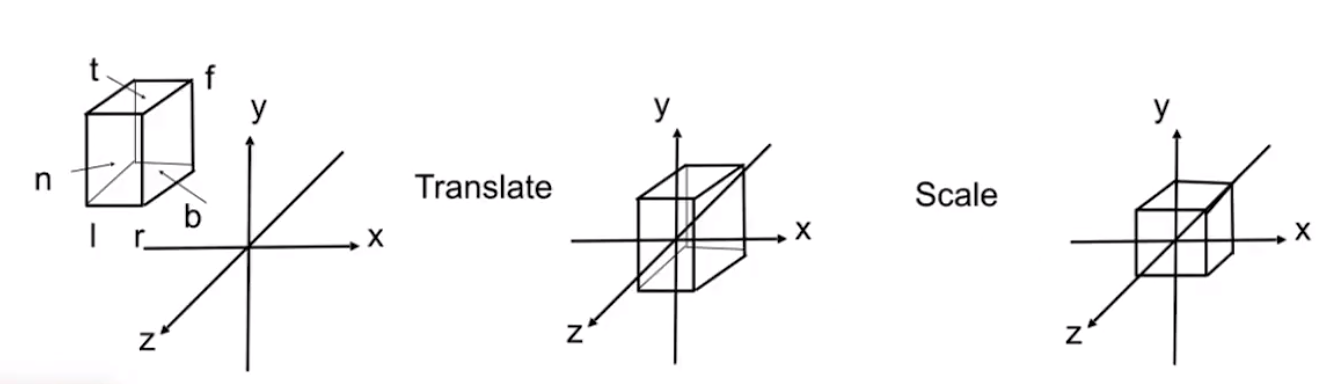
\includegraphics[scale=0.5]{resources/OrthographicProjection.png}

                        矩阵形式为:$$
                          M_{ortho} = \begin{bmatrix}
                            \cfrac{2}{r - l} & 0                & 0                & 0 \\
                            0                & \cfrac{2}{t - b} & 0                & 0 \\
                            0                & 0                & \cfrac{2}{n - f} & 0 \\
                            0                & 0                & 0                & 1
                          \end{bmatrix}
                          \begin{bmatrix}
                            1 & 0 & 0 & -\cfrac{r + l}{2} \\
                            0 & 1 & 0 & -\cfrac{t + b}{2} \\
                            0 & 0 & 1 & -\cfrac{n + f}{2} \\
                            0 & 0 & 0 & 1
                          \end{bmatrix}
                        $$

                        \begin{itemize}
                          \item 注意:由于视线方向沿着-z,所以$n>f$
                          \item 这就是为啥OpenGL用的是左手系
                        \end{itemize}
                        }
                  \item {
                        透视变换(Perspective projection) :

                        首先把视锥压缩成长方体.(近平面永远不变,远处平面z值不发生变化,中心点不发生变化)$(n \to n,f \to f,M_{persp \to ortho})$

                        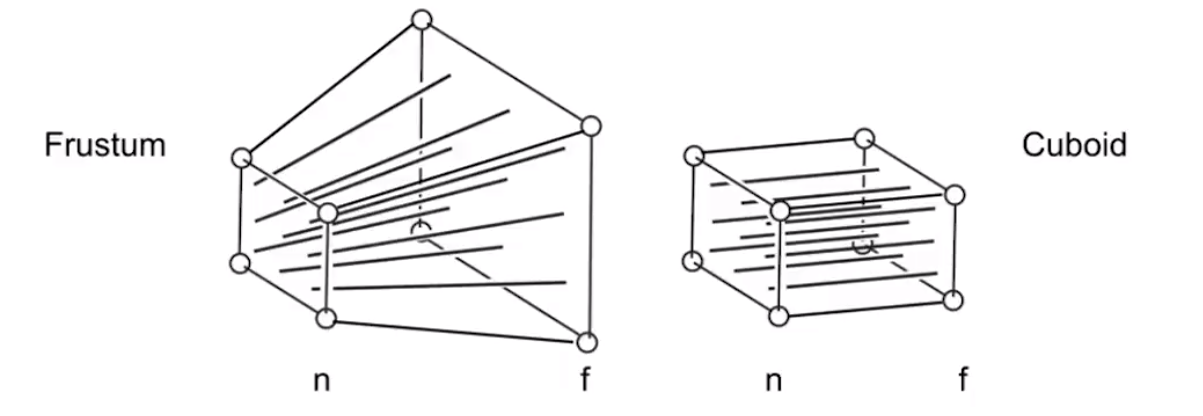
\includegraphics[scale=0.5]{resources/perspectiveProjection.png}

                        关键就在于:要找到中点和被投影对象之间的联系.

                        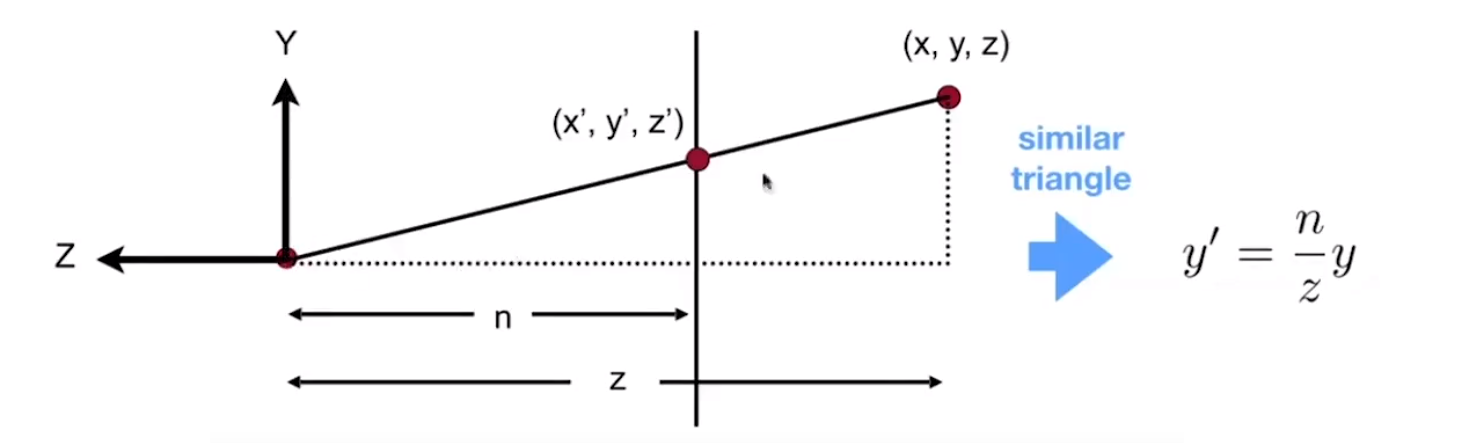
\includegraphics[scale=0.5]{resources/perspectiveProjection_middle.png}

                        $y^\prime = \cfrac{n}{z}y$,由这个公式就可以算出来压缩后的y,并且结果是满足要求的.

                        类似的,还有$x^\prime = \cfrac{n}{z}x$

                        于是得出结论:$$
                          \begin{bmatrix}
                            x \\
                            y \\
                            z \\
                            1
                          \end{bmatrix}
                          \Rightarrow
                          \begin{bmatrix}
                            \cfrac{nx}{z} \\
                            \cfrac{ny}{z} \\
                            unknow        \\
                            1             \\
                          \end{bmatrix}
                          ==
                          \begin{bmatrix}
                            nx           \\
                            ny           \\
                            still unknow \\
                            z
                          \end{bmatrix}
                        $$
                        因此,透视变换的本质就是由目标平面和被投影平面构造一个直角三角形

                        由此写出未完成的投影矩阵 : $$
                          M_{persp \to ortho}
                          =
                          \begin{bmatrix}
                            n & 0 & 0 & 0 \\
                            0 & n & 0 & 0 \\
                            ? & ? & ? & ? \\
                            0 & 0 & 1 & 0
                          \end{bmatrix}
                        $$

                        而这一行未知的也一定与z有关系.

                        另外,任何在目标平面上的点被投影后一定在原地,也就是说:$$
                          \begin{bmatrix}
                            x \\
                            y \\
                            n \\
                            1
                          \end{bmatrix}
                          \Rightarrow
                          \begin{bmatrix}
                            x \\
                            y \\
                            n \\
                            1
                          \end{bmatrix}
                          ==
                          \begin{bmatrix}
                            nx  \\
                            ny  \\
                            n^2 \\
                            n
                          \end{bmatrix}
                        $$

                        仔细思考可以得出:矩阵第三行前两个未知数一定为0:$$
                          \begin{bmatrix}
                            0 & 0 & A & B
                          \end{bmatrix}
                          \begin{bmatrix}
                            x \\
                            y \\
                            n \\
                            1
                          \end{bmatrix}
                          =
                          n^2
                        $$

                        结合另一件事 : 被投影平面上的中心点投影后位置不变,可得出:$$
                          \begin{cases}
                            \begin{bmatrix}
                              0 & 0 & A & B
                            \end{bmatrix}
                            \begin{bmatrix}
                              x \\
                              y \\
                              n \\
                              1
                            \end{bmatrix}
                            =
                            n^2
                            \rightarrow
                            An + B = n^2 \\
                            \begin{bmatrix}
                              0 \\
                              0 \\
                              f \\
                              1
                            \end{bmatrix}
                            \Rightarrow
                            \begin{bmatrix}
                              0 \\
                              0 \\
                              f \\
                              1
                            \end{bmatrix}
                            ==
                            \begin{bmatrix}
                              0   \\
                              0   \\
                              f^2 \\
                              f
                            \end{bmatrix}
                            \rightarrow
                            Af + B = f^2
                          \end{cases}
                          \rightarrow
                          \begin{cases}
                            A = n + f \\
                            B = -nf
                          \end{cases}
                        $$
                        所以 : $$
                          M_{persp \to ortho}
                          =
                          \begin{bmatrix}
                            n & 0 & 0     & 0   \\
                            0 & n & 0     & 0   \\
                            0 & 0 & n + f & -nf \\
                            0 & 0 & 1     & 0
                          \end{bmatrix}
                        $$

                        最后将正交投影和此式结合起来使矩阵变得完整 : $M_{persp} = M_{ortho}M_{persp \to ortho}$
                        }
                \end{itemize}
                }
        \end{itemize}


      }%观测变换结尾

    }%变换结尾

   }%计算机图形学结尾

  \section{硬件}{

   }%硬件结尾

  \section{网络通信}{

   }%网络通信结尾

  \section{科研辅助}{

   }%科研辅助

 }%计算机科学篇结尾

\chapter{逻辑学}{

  \section{逻辑学基本常识}{

    \subsection{充分必要条件}{

      充分必要条件(sufficient and necessary condition)简称为充要条件.

      在逻辑学中:
      \begin{itemize}
        \item 当命题"若P则Q"为真时,P称为Q的充分条件,Q称为P的必要条件.

              因此:

        \item 当命题"若P则Q"与"若Q则P"皆为真时,P是Q的充分必要条件,同时,Q也是P的充分必要条件.
        \item 当命题"若P则Q"为真,而"若Q则P为假时",P是Q的充分不必要条件,Q是P的必要不充分条件,反之亦然.
      \end{itemize}

      \subsubsection{必要条件}{
        P是Q的必要条件,代表"如果P是假,则Q是假"

        以逻辑符号表示:

        $\lnot P \to \lnot Q$

        通过否定后件,得出"如果Q是真,则P是真".

        $Q \to P$
      }%必要条件结尾

      \subsubsection{充分条件}{
        P是Q的充分条件,代表"如果P是真,则Q是真"或"如果Q是假,则P是假".

        以逻辑符号表示:

        $P \to Q$
      }%充分条件结尾

      \subsubsection{必要条件及充分条件}{
        P是Q的充分及必要条件,代表"当且仅当P是真,则Q是真".

        以逻辑符号表示:

        $P \longleftrightarrow Q$

        留意$\lnot P \to \lnot Q$可以推出$Q \to P$.

        $(\lnot P \to \lnot Q) \land (P \to Q)$

        $(Q \to P) \land (P \to Q)$

        $P \longleftrightarrow Q$
      }%必要条件及充分条件结尾

    }%充分必要条件结尾

   }%逻辑学基本常识结尾

 }%逻辑学结尾


\end{document}